\documentclass[a4paper,fleqn]{cas-dc}
\usepackage[numbers]{natbib}
\usepackage{amsmath,amsfonts}
\usepackage{algorithm}
\usepackage{algorithmic}
\usepackage{array}
\usepackage[caption=false,font=normalsize,labelfont=sf,textfont=sf]{subfig}
\usepackage{textcomp}
\usepackage{stfloats}
\usepackage{url}
\usepackage{verbatim}
\usepackage{graphicx}
\hyphenation{op-tical net-works semi-conduc-tor IEEE-Xplore}
\def\BibTeX{{\rm B\kern-.05em{\sc i\kern-.025em b}\kern-.08em
    T\kern-.1667em\lower.7ex\hbox{E}\kern-.125emX}}
\usepackage{balance}
\begin{document}
\let\WriteBookmarks\relax
\def\floatpagepagefraction{1}
\def\textpagefraction{.001}

\shorttitle{Embedded Ray-Traced Propagation for ns-3}
\shortauthors{Aung Kaung Myat et al.}

\title[mode = title]{Embedded Ray-Traced Propagation for End-to-End 6G Packet-Level Simulation in ns-3}

\author[1]{Aung Kaung Myat}
\cormark[1]
\ead{aung-kaung.myat@telecom-sudparis.eu}

\author[1]{Hrishikesh Dutta}
\ead{hrishikesh.dutta@telecom-sudparis.eu}

\author[1]{Roberto Minerva}
\ead{roberto.minerva@telecom-sudparis.eu}

\author[1]{Djamal Zeghlache}
\ead{djamal.zeghlache@telecom-sudparis.eu}

\author[1]{Noel Crespi}
\ead{noel.crespi@telecom-sudparis.eu}

\affiliation[1]{organization={SAMOVAR, Télécom SudParis, Institut Polytechnique de Paris},
    addressline={},
    city={Palaiseau},
    country={France}}

\cortext[1]{Corresponding author}

\begin{abstract}
System-level network simulators such as ns-3 model the protocol stack with high fidelity but rely on analytical propagation models -- Friis, log-distance, 3GPP TR~38.901 stochastic -- that cannot reproduce environment-specific effects critical to 5G/6G physical-layer studies. Conversely, modern differentiable ray tracers such as Sionna~RT capture site-specific multipath, polarization, and antenna geometry but lack a discrete-event protocol stack. We present \emph{sionnart}, an ns-3 contrib module that embeds Sionna~RT directly into the simulator's address space via pybind11 and exposes it through standard \texttt{PropagationLossModel}, \texttt{PropagationDelayModel}, and \texttt{SpectrumPropagationLossModel} interfaces. A coherence-aware cache validated by a wavelength-and-array-derived displacement bound $\delta = \max(\delta_\mathrm{min}, \alpha\, d \cdot 0.886 / N_\mathrm{cols})$, coupled with a proactive virtual receiver generation mechanism that samples future channel states along mobile trajectories, suppresses redundant ray-tracer invocations while preserving channel realism. We evaluate sionnart in two campaigns: (i)~against the prior socket-coupled ns3sionna and a pure-ns-3 Friis baseline on an 802.11ax scenario across station counts $N \in \{1,\ldots,32\}$ and three mobility/load regimes; sionnart is up to ${\sim}232\times$ faster than ns3sionna at $N{=}32$ stationary load and ${\sim}44\times$ faster under high mobility while maintaining a minimal, flat GPU footprint under 500~MiB. It is even ${\sim}40\times$ faster than pure ns-3 in the stationary regime because cache hits replace recomputation. (ii)~On a 5G LENA NR setup with planar arrays $\{2{\times}2, 4{\times}4, 8{\times}8\}$ across free-space, urban-micro, and urban-macro scenes under three traffic loads. We demonstrate that deterministic multipath fading enforces more conservative, realistic CQI/MCS scheduling than stochastic models. This channel realism significantly shifts downstream metrics, altering gNB power consumption by up to $-29\%$ and uplink throughput by up to $+55\%$ relative to the analytical baseline, highlighting critical throughput and energy consumption trade-offs when scaling array sizes in complex environments. The artifact is a reusable contrib module and a methodology for fast, repeatable ray-traced network experiments suitable for digital-twin applications.
\end{abstract}

\begin{IEEEkeywords}
ns-3, Sionna~RT, ray tracing, 5G NR, energy modeling, propagation cache, network simulation, digital twin.
\end{IEEEkeywords}


\maketitle


\section{Introduction}

Sixth-generation cellular and next-generation wireless local-area networks are increasingly defined by their interaction with the radio environment rather than by abstract path-loss exponents. Joint communication and sensing, integrated access and backhaul, reconfigurable intelligent surfaces, and AI-driven beam management all require simulation tools that can resolve geometry, materials, and antenna directivity at the level of individual rays. At the same time, the network and transport behavior that determines user-perceived performance -- random access, scheduling, hybrid ARQ, congestion control, mobility procedures -- lives several layers above the physical channel and is most faithfully captured by discrete-event simulators with mature protocol stacks.

ns-3 is the de facto open-source platform for that protocol-stack fidelity. It ships with a modular contrib system, a stable C++ API for propagation and spectrum models, and an actively maintained 5G NR module (5G LENA). Its propagation models, however, are by design mathematically tractable rather than environment-specific: Friis, log-distance, 3GPP TR~38.901 spatial-channel models, and a handful of empirical alternatives. None capture the deterministic multipath structure of a particular factory floor or city block.

NVIDIA's Sionna~RT is, conversely, a state-of-the-art differentiable ray tracer with first-class support for planar antenna arrays, dual polarization, and scene loading. It is, however, a Python library oriented around standalone link-level studies; it does not implement MAC, RLC, PDCP, or any network protocol.

Bridging the two has historically meant \emph{socket-coupling}: launching the ray tracer as a separate process and exchanging position and channel data over ZMQ or TCP. The reference implementation \texttt{ns3sionna} follows this pattern, and our own measurements (Section~\ref{sec:results}) confirm that under mobility-dominated load it imposes prohibitive overhead -- wall-clock times in the tens of minutes for ten seconds of simulated time at modest user counts. The cost is dominated not by ray tracing itself but by per-step IPC, serialization, and the absence of a shared cache state between the two address spaces.

This paper contributes:

\begin{enumerate}
\item \textbf{An embedded integration}, \texttt{contrib/sionnart}, in which the Python interpreter and Sionna~RT live inside the ns-3 process via pybind11. C++ propagation models call Python directly, circumventing expensive IPC overheads and enabling a shared memory space.
\item \textbf{A displacement-based coherence-aware cache and proactive virtual receiver generation.} To further minimize computationally expensive ray-tracing calls, we introduce a cache whose validity bound is mathematically tied to spatial displacement and array geometry, coupled with an adaptive mechanism that samples future channel states along a mobile node's predicted trajectory.
\item \textbf{An evaluation across two experimental campaigns.} Campaign~I quantifies the runtime advantages of our architecture, demonstrating up to a $232\times$ speedup over socket-coupled designs while maintaining a minimal, flat GPU memory footprint under high-mobility loads. Campaign~II examines the impact of channel realism on 5G NR networks across free space, urban macro, and urban micro environments. It reveals how deterministic multipath fading enforces more conservative, realistic CQI/MCS scheduling than stochastic models, fundamentally shifting throughput and energy consumption trade-offs when scaling massive MIMO arrays up to $8\times8$.
\end{enumerate}

The remainder of the paper is organized as follows. Section~\ref{sec:litreview} reviews related simulation platforms and motivates ns-3 as the host. Section~\ref{sec:methodology} describes the system architecture, cache mechanism, adaptive virtual receiver generation, and the NR energy formulation. Section~\ref{sec:results} reports experimental results from both campaigns. Section~\ref{sec:conclusion} discusses limitations, concludes, and outlines future work.


\section{Background}
\label{sec:litreview}

To understand the motivation behind the integration of ns-3 and Sionna RT, this section reviews the evolution toward Massive MIMO and the need for physically realistic channel models in 6G systems research.
The difference between traditional stochastic approaches and deterministic ray-tracing approache is discussed, hightlighting the need for the latter in 6G systems research.
Finally, discuss the limitations of prior integration with Simu5G and motivates the use of ns-3 combined with Sionna RT to achieve realistic channel modelling and computationally efficient simulations for advanced 6G research.

\subsection{Massive MIMO for 6G}
Multiple-Input Multiple-Output (MIMO) technology is a fundamental building block of 6G systems \cite{bojovic_mimo,cazzella_dt_mimo}.
Large scale MIMO antenna arrays are essential for operating in high-frequency bands such as mmWave and THz \cite{uwaechia_mmwave,han_thz}.
With the evolution of MIMO antenna arrays, they were able to provide highly directional beamforming and increased angular resolution, allowing the network to distinguish users and objects in environment \cite{bojovic_beamforming,gao_isac_mimo}.
This capabilities are important for emerging 6G applications where it has operate in complex, dynamic environment.

In particular, MIMO plays a improtant role in Integrated Sensing and Communication (ISAC), where wireless channel is exploited not only for data transmission but also for environment sensing \cite{zhou_isac,gao_isac_mimo,hua_isac_beamforming}.
In such systems, spatial information of channel such as angles, delays, etc carry information about the physical environment including position and movment of objects.
Capturing accurately of these information is critical for enabling functionalities such as beam tracking, object detection, and context-aware decision-making.

However, testing and deploying such kind of systems in real world is challenging due to high cost, complex setup, and limited availability of testing facilities.
Simulation become important to overcome these limitation for 6G research.
It provide a controlled and scalable environment to evaluate advance MIMO techniques under realistic conditions.
However, conventional stochastic channel models, that are widely use in simulators, are designed for statical performance evaluation and lack geometric information required for application such as ISAC \cite{tr38901,alsamman_mmwave,han_thz}.
This limitation movitates the adoption of physically grounded simulation approaches that can accurately represents the interaction between electromagnetic waves and the environment.


\subsection{Stochastic vs Deterministic Channel Modeling}
Channel modeling can be broadly classified into two categories, namely stochastic and deterministic channel modeling.
Stochastic models rely on satistcial distributions to represent large-scale effects such as path loss and shadowing as well as small-scale fading through multipath clusters \cite{tr38901}.
These models are computationally efficient and widely adopted in system-level simulators to evaluate average network performance across standardized deployment scenarios \cite{tr38901,5glena}.

Eventhough they are suitable for lage-scale evalution, they lack site-specific realistic geometric information about the environment \cite{alsamman_mmwave,han_thz}.
For instance, a stochastic model cannot distinguish between a line-of-sight path along an open space and blocked path behind a building as both are represented through probalistic parameters.
In constrast, deterministic modeling computes the actual electromagnetic interactions within a given 3D environment.

While full-wave solutions based on Maxwell's equations are computationally infeasible, high-frequency approximations such as ray-tracing provide a pratical alternative \cite{alsamman_mmwave,han_thz}.
Ray-tracing bridges the gap between statistical averages and physical reality by resolving propagation paths including reflections, diffrations and blockages.
This is especially important for 6G research as they use mmWave and THz frequency bands, where propagation is highly directional and sensitive to enviorment geometry \cite{uwaechia_mmwave,han_thz}.


\subsection{Ray-Tracing based Simulation}
Ray-tracing is a deterministic channel modeling technique that provides a physically grounded representation of radio signal propagation.
It models how electromagneticwaves interact with the enviroment by considering refelction, diffrations, and scattering.

The fundamental principle of ray-tracing is to approximate electromagnetic waves as rays whose paths are geometrically computed.
The channel repose between a transmitter and a receiveris derived by tracing multiple propagation of emitted rays which interact with surronding objects, undergoing reflections, diffractions, or scattering based on the material and geometry of enviroment.
Ray-tracing has been widely used sicne 1990s for modeling radio propagation in complex environments.
Its deterministic nature enable high accuracy in predicting signal strength, delay spread, and angle of arrival, which are crucial for advanced wireless communication systems.

Main advantage of ray-tracing over traditional stochatic models is its ability to provide site-specific realistic channel modeling.
This property enables channel evolves smoothly with user modiblity, making it suitable for evaluating advanced scenarios that are difficult to capture with stochatic models.
For example, ray-tracing can accurately capture the signal drop when a user moves behind a building, which is difficult to model with traditional stochastic approaches.
Furthermore, ray-tracing can provide detailed spatial information about the propagation environment, such as angle of arrival and delay spread, which are crucial for advanced wireless communication systems.

Despite its advantages, ray-tracing is computationally expensive due to the need to evaluate a large number of propagation paths.
Recent advances in computing hardware, especially the use of GPUs and parallel processing techniques, have made ray-tracing more practical for large-scale simulations.

\subsection{Simu5G and Sionna Prior Integration Limitations}
Simu5G\cite{simu5g} is an open-source 5G system-level simulator built on the OMNeT++ framework. It is developed by a consortium of universities and research centers in Spain, led by the Universitat Politècnica de Catalunya (UPC) and has been used for various research works on 5G networks.

Simu5G use Network Description language (NED) for topology and C++ for behavior of the network and applications. Topology is defined in NED file, parameters are passed through a separate omnetpp.ini file and instantiated via a runtime that reflects on those declarations.
While elegant for purely C++ network research, the framework is very rigid and hard to integrate with other frameworks such as SionnaRT which is based on Python.

Another key limitation of Simu5G is its lack of native support for multi-input multi-output (MIMO) antenna systems.
Recent versions of Simu5G doesn’t support MIMO antenna systems natively and require workarounds to enable it which
add another layer of complexity and brittleness to the framework.

In addition, it use statistical models for channel modeling which are not as accurate as ray-traced models that reflect the physical environment. Propagation loss and delay are modeled stochastically, which can be acceptable
for large-scale system-level analysis but is inadequate for high-accuracy simulations of dense urban or indoor environments.
Despite our previous efforts to integrate SionnaRT with Simu5G for MIMO antenna systems with ray-tracing capabilities, we encountered several limitations that motivated our transition to ns-3 for our 6G simulations.
Transitioning to ns-3 significantly provide multiple advantages including easier integration with other frameworks such as SionnaRT which is based on Python, native support for MIMO antenna systems and ability to use thirty party libraries like 5G LENA NR for 5G NR simulations.

\subsection{ns3}
ns-3 is an open-source, discrete-event network simulator developed in C++ with support for integration with Python \cite{ns3}.
It is an end-to-end network simulator, alternative to OMNeT++, and is widely used in academic for research of communication networks.
ns-3 is developed to reflect the reality as close as possible with core concepts and abstractions that map closely to how the real communication network are built.

In ns-3, a \texttt{Node} is a fundamental network entity. It serves as a container for \texttt{Application}, \texttt{Protocols}, and \texttt{Network Devices}.
Each node can run an \texttt{Application} which is a user program that generate packet flows.
Ns-3 has several built-in traffic generator for different applications such as video streaming, social media, gaming, VoIP, FTP, etc.

A \texttt{Network Device} is an entity that connected to a \texttt{Channel} which represent the transmission medium between the devices.
The broad community has continuously contributed to the network simulator, which now supports different channel models such as Ethernet, Wi-Fi, LTE, WiMax, etc. \cite{ns3}.
Each time a node sends a packet, the \texttt{Channel} calls a statistical or stochastic model, such as Friis, Log-Distance, or 3GPP \texttt{Propagation\allowbreak LossModel} and \texttt{Propagation\allowbreak DelayModel}, to calculate the path loss and transmission delay for that particular transmission \cite{ns3,tr38901}.

Moreover, ns-3 provide mobility model such as \texttt{ConstantPositionMobilityModel} and \texttt{RandomWalk2MobilityModel} to simulate the movement of devices.
However, the propagation models provided in ns-3 are limited to statistical models and support for 5G NR and beyond is not supported yet in main framework.


\subsection{5G LENA NR Module}
5G-LENA NR \cite{5glena} is an extension of ns-3 developed by CTTC for simulating 3GPP compliant 5G NR cellular networks across both  sub-6 Hz and mmWave frequency ranges (0.5 to 100 GHz).
The module implements  5G NR core network components, protocol stack including the Physical (PHY), Medium Access Control (MAC), Radio Link Control (RLC), and Packet Data Convergence Protocol (PDCP) layers.
The MAC layer in 5G-LENA supports flexible schedulers (e.g., Proportional Fair, Round Robin) for both TDMA and OFDMA-based access, while the PHY layer handles advanced MIMO models and MCS (Modulation and Coding Scheme) adaptation.

While 5G-LENA NR provides the protocol stacks for 5G NR, it still rely on the standard ns-3 propagation models which cause the same limitations previously discussed.
Specifically, it lacks the site-specific channel information related to environment that it is deployed in.
Such information are important to model different research scenarios such as ISAC in 6G network systems.
This gap in physical-layer realism is the final motivator for us to integrate a ray-tracing engine into 5G-LENA NR.

\subsection{Sionna RT}
Sionna version two is a hardware-accelerated differentiable open-source library for research on communication systems \cite{sionna,sionnart}.
It is built on top of Mitsuba 3 and Dr.JIt while the API is written in PyTorch unlike the original Sionna library.
It is composed of \texttt{Sionna RT} which is a stand-alone ray tracer for radio propagation modelling, \texttt{Sionna PHY}, a link-level simulator for wireless and optical communication and \texttt{Sionna SYS}, system-level simulation functionalities based on physical-layer abstraction \cite{sionna,sionnart}.

However, it lacks the functionalities to simulate the whole 5G NR protocol stack \cite{sionna,sionnart,5glena}. This is where ns-3 comes in.
Sionna RT provides the realistic channel modelling which reflect the propagation of radio waves in a given environment while ns-3 provides the functionalities to simulate the remaining part of the 5G NR protocol stack.
To integrate the Sionna RT into ns-3, we leverage pybind11, allowing Sionna RT to live directly within the ns-3 process \cite{pybind11,sionna,sionnart}.
This allows the simulator to calculate spatially consistent CIRs with minimum overhead, effectively replacing stochastic abstractions with deterministic physical calculations.


\section{Methodology}
\label{sec:methodology}

The overall architecture of the proposed integrated simulation framework is depicted in Figure \ref{fig:system_architecture}.
The proposed integrated simulation framework follows a layered design in which ns-3 remains the primary discrete-event simulator while Sionna RT is embedded as environment aware ray-tracing engine.
The main goal of the architecture is to preserve the mature protocol, traffic generation, scheduling capabilities of ns-3, Sionna RT handle ray-tracing which provide realistic site-specific propagation channel model, while leveraging GPU acceleration for computation intensive process

\begin{figure}[htbp]
    \centering
    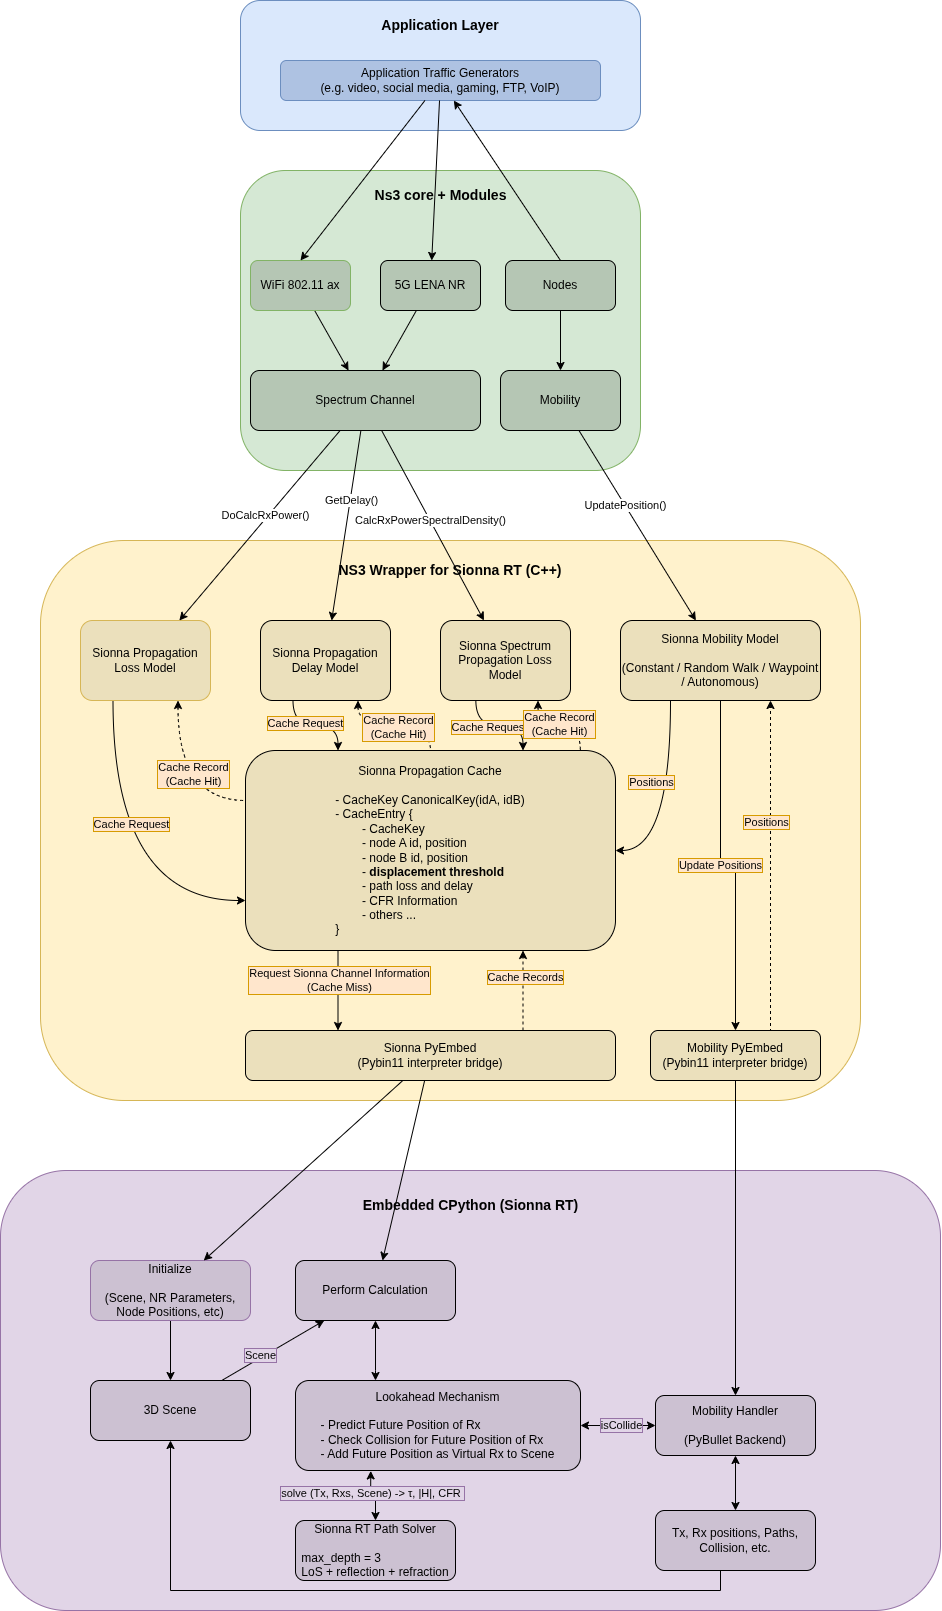
\includegraphics[width=\linewidth]{images/SionnaRT_System_Architecture.drawio.png}
    \caption{Architecture of the integrated simulation framework. }
    \label{fig:system_architecture}
\end{figure}

At the top is the application layer where the user defined traffic are generated between UEs and gNB.
These traffic can be of different type such as video streaming, social media, gaming, FTP and VoIP.
This traffic generators allow to simulate different workload scenarios which reflect the realistic network traffic behavior.

The middle layer colored in green is the network layer where the ns-3 stack is located.
Node manangement, mobility, routing, scheduling are handled by this layer.
It also handle MAC layer operation according to the chosen medium access and protocol standard.
For instance, the way packet processed for Wi-Fi 802.11ax or 5G NR is different and it is handled by the ns-3 MAC layer.
When a packet is generated by the application layer, it is first passed to the ns-3 stack.
Then, the ns-3 stack processes the packet according to the protocol stack.
Finally, the packet is transmitted over the wireless medium where it call \texttt{PropagationLossModel} and \texttt{PropagationDelayModel}, in order to calcualte path loss, transmission delay and channel fade.

When the call to \texttt{PropagationLossModel} and \texttt{PropagationDelayModel} triggered, the compuation of propagation delay and path loss is handled by the Sionna RT engine which provide environment aware channel information.
However, compuation these information using ray-tracing every time packet traverses is computationally intensive and it can significantly slow down the simulation.
To address this challenge, the next layer handle this issue using caching mechanism.
Whenever, a packet traverses between node A and node B, it check in cache for the channel information using their positions.
If the nodes are in positions where the calculated dispalcement distance is below the threshold value, it retrieve the channel information from cache as channel information relatively unchanged if they are under the coherence distance.
Otherwise, it trigger the ray-tracing engine to compute the channel information and update the cache with the new information.
In order to maximize the caching efficiency and reduce number to times it has to call the ray-tracing engine, future possible positions of the nodes are generated based on their current position and speed.

Then these generated positions are added to the scene as virtual receviers in additional to real receviers and the paths calculation is done by Sionna RT engine for all  receviers (real and virtual).
The channel information obtained for virtual receviers are added to the cahce for future use in addition to the channel information of the real positions.
This help to remove the need to call the ray-tracing engine every time packet traverses.
However, ns-3 can not directly call the Sionna RT engine to compute the channel information as they are written in different programming languages.
So, wrapper class is created to call Sionna RT engine from ns-3 in this layer.

Final bottom most layer which is in purple color is the Sionna RT engine where the ray-tracing is performed to compute the channel information.
Before the simulation starts, the radio propagation parameters, antenna configuration, and 3D scene information are initlized by passing the information form ns-3 side.
During the simulation, when the channel information requested is not in the cache, the calculation for future positions of the node, channel information for each node in different positions is calculated by using Sionna Path Solver.
Path solver calculate path loss, time of arrival, angle of arrival, angle of departure, etc based on the rays propagated in the 3D environment.
These calculation are done on GPU for efficient computation which give substantial performance.
Finally, the calculated channel information is returned to the ns-3 side through the wrapper class and updated in the cache.


\subsection{Sionna Propagation Cache Mechanism}
\label{sec:sionna-cache-mechanism}

\subsubsection{Displacement-Based Cache Validity}
\label{subsec:cache-validity}

Performing the calculation using ray-tracing on Sionna RT is an computationally intensive calculation.
The goal of the cache mechanism is to reduce this computationally expensive calculation for every ns-3 propagation query.
When the receiver moved only a small distance from the previous position, the propagation information does not change significantly.
By using this idea, the cache validation is implemented based on spatial displacement rather than a fixed time interval.
In this section, how the cache is implemented is described in detail.

The cache stores the records of the each transmitter and receiver pair for ns-3 simulation.
Each cache entry is indexed by a canonical unordered node pair,
\begin{equation}
    \kappa(a,b)=\left(\min(I_a,I_b),\max(I_a,I_b)\right),
\end{equation}
where $I_a$ and $I_b$ are ns-3 node identifiers.
During the runtime, the cache stores the node positions $\mathbf{x}_a^0$ and $\mathbf{x}_b^0$, path loss, transmission delay, channel frequency reqponse (CFR), and the state for path whether it is in Line of Sight (LoS).

The distance between Tx and Rx is calculated using
\begin{equation}
    d_{a,b}^0=\left\|\mathbf{x}_a^0-\mathbf{x}_b^0\right\|_2 ,
\end{equation}
and the validity radius can be calculated using
\begin{equation}
    \Delta_{a,b}=
    \max\left(
    \Delta_{\min},
    \alpha \frac{0.886 d_{a,b}^0}{N_{\mathrm{tx,col}}}
    \right).
\end{equation}
where $\alpha$ is set to $0.4$ and $\Delta_{\min}$ is set to $0.1$ m as default values.

When the query for propagation delay and path loss happens for the Tx-Rx pair, the current posisitons  $\mathbf{x}_a(t)$ and $\mathbf{x}_b(t)$
are compared against the trace-time positions.
A valid cache entry is found if
\begin{equation}
    \left\|\mathbf{x}_a(t)-\mathbf{x}_a^0\right\|_2 < \Delta_{a,b}
    \quad\mathrm{and}\quad
    \left\|\mathbf{x}_b(t)-\mathbf{x}_b^0\right\|_2 < \Delta_{a,b}.
\end{equation}.
Ifboth inequalities are satisfied, the propagation delay and path loss and other data are returned directly.
Otherwise, the cache lookup is considered as a cache miss and the snapshot is refreshed.

\subsubsection{Snapshot Refresh}
\label{subsec:cache-refresh}

When the cache miss happen, it does not referesh only one link between Tx and Rx.
Instread, it refreshes the cache for all Tx-Rx pairs.
First, positions of every node which are using \texttt{SionnaMobilityModel} are synchronized into the Python Sionna scene.
Then it performs one batched calculation using ray-tracing for all Tx-Rx pairs by invoking \texttt{perform\_calculation} in \texttt{sionnart.py}.
This is designed in such a way to reduce overall computation using ray-tracing by calculating for all Tx-Rx pairs at once.
When the calculation are completes, it converts the returned records through pybind, and inserts them as new cache records in ns-3 propagation cache.
For each record, the cache stores
\begin{equation}
    \left(
    \tau_{a,b},\,
    L_{a,b},\,
    \mathbf{h}_{a,b},\,
    \mathbf{H}_{a,b},\,
    \mathbf{f},\,
    \mathrm{LoS}_{a,b},\,
    \mathbf{x}_a^0,\,
    \mathbf{x}_b^0,\,
    \Delta_{a,b}
    \right),
\end{equation}
where $\tau_{a,b}$ is delay, $L_{a,b}$ is path loss, $\mathbf{h}_{a,b}$ is the
scalar CFR, $\mathbf{H}_{a,b}$ is the MIMO CFR, and $\mathbf{f}$ is the
frequency vector.
The old cache records are removed only if the new results contains usable records.

\subsubsection{Lookup and Fallback Behavior}
\label{subsec:cache-lookup-fallback}

ns-3 query propagation related information for each Tx and Rx pair.
For a normal link, the cache lookup sequence is that it search the canonical key, test displacment validity, and return the first valid entry it found.
If no valid entry exists, the cache refreshes the full records and retris the same lookup sequence.

In Sionna RT, the link between nodes with same radio role, such as Tx--Tx or Rx--Rx, are not computable.
In such cases, the dummy entry with large path loss and delay are returned instead.
If Sionna RT does not return usable data for the requested link after refresh, the cache falls back to stochastic Friis model and constant constant-speed delay are returned for that lookup.

Moreover, before calling Sionna RT to refresh the cache, it checks estimated received power using Friis in order to avoid unnecessary computation expensive calculation.
If
\begin{equation}
    P_{\mathrm{Friis}}^{\mathrm{rx}} + M
    <
    P_{\mathrm{weak}},
\end{equation}
where $P_{\mathrm{weak}}=-95$ dBm and $M=6$ dB by default, the link is treated
as too weak to justify ray tracing.
In that case,  Friis loss and constant-speed delay are used directly.

\subsubsection{Derived MIMO Caches}
\label{subsec:derived-mimo-caches}

The cache records returned from Sionna side stores the normalized element-level MIMO CFR.
However, ns-3 needs derived quantities such as  port-level channel, matrices, PSD-scaled matrices, and effective gains after precoding.
These quantities depend not only on geometry but also on antenna objects, beamforming vectors, PSDs, and precoders.
Thus, these information are computed based on the returned element-level MIMO CFR and other information from the ns-3 side, and stored in the propagation entry as derived quantities.

The calculation can be done as followed.
For a given beam configuration, the element-level channel is projected onto
antenna ports.
For resource block $q$, transmit port $p_t$, and receive port
$p_r$, the port-level channel has the form
\begin{equation}
    G_{p_r,p_t}[q]
    =
    \sum_{i\in\mathcal{E}_{p_r}}
    \sum_{j\in\mathcal{E}_{p_t}}
    w_{r,i}\,w_{t,j}\,
    \widetilde{H}_{i,j}[q],
\end{equation}
where $\mathcal{E}_{p_r}$ and $\mathcal{E}_{p_t}$ are the receive and transmit
element sets associated with the ports, and $w_{r,i}$ and $w_{t,j}$ are the
beamforming weights.
This port CFR is cached using antenna identifiers,
beamforming-vector hashes, port counts, and link direction.

For spectrum propagation, the port CFR is scaled by the input PSD:
\begin{equation}
    C_{p_r,p_t}[q]
    =
    \sqrt{S[q]}\,G_{p_r,p_t}[q],
\end{equation}
where $S[q]$ is the PSD value on resource block $q$. The most recent
PSD-scaled matrix is cached using a PSD hash and PSD size.

When a precoding matrix $\mathbf{W}[q]$ is provided, the effective gain per
resource block is
\begin{equation}
    g[q]
    =
    \sum_{p_r}\sum_s
    \left|
    \sum_{p_t} G_{p_r,p_t}[q] W_{p_t,s}[q]
    \right|^2 .
\end{equation}
These gains are cached using the port-CFR key, precoder hash, precoder
dimensions, and output resource-block count.
This avoids repeated beamforming and precoding reductions while the underlying propagation entry remains valid.


\subsection{Adaptive Virtual Receiver Generation}
\label{subsec:adaptive-virtual-rx-generation}

The coherence cache described in Section~\ref{sec:sionna-cache-mechanism} is reactive: a new ray tracing call is issued only after a cache entry becomes invalid.
Adaptive virtual receiver generation is a complementary proactive mechanism that reduces the number of such cache misses.
During each cache refresh, a small number of temporary receiver positions are placed ahead of each UE along its trajectory.
These positions are not new network nodes; they are spatial samples for the same UE at predicted future locations.
Including them in the same Sionna RT call returns both present and near-future channel samples at no additional ray tracing overhead.

Let the UE position and speed be
\begin{equation}
    \mathbf{x}_r(t)=[x_r(t),y_r(t),z_r(t)]^{\mathsf{T}},
    \qquad v_r .
\end{equation}
Prediction of virtual receiver positions is not performed for a stationary receiver (i.e., $v_r \leq 10^{-6}$~m/s).
For a moving UE, the distance to the nearest transmitter is
\begin{equation}
    d_r(t)=\min_{b\in\mathcal{B}}
    \left\|\mathbf{x}_r(t)-\mathbf{x}_b\right\|_2 .
\end{equation}
The valid displacement $\Delta_r$ is computed using the coherence formula
from Section~\ref{subsec:cache-validity}, based on $d_r(t)$ and a default
$\Delta_{\min}=0.5$ m.
The current sample is predicted to expire after
\begin{equation}
    T_{\mathrm{expire},r}=\frac{\Delta_r}{v_r}.
\end{equation}
This is the time for the UE to travel the full valid displacement at its current speed.
Virtual receivers are generated only if $T_{\mathrm{expire},r}<T_{\min}$, with $T_{\min}=1$ s.

The generation of virtual receivers is closely tied to the underlying mobility model of the UE.
For UEs with predictable trajectories, such as those using a Waypoint mobility model, the direction of motion is stable and virtual receivers are reliably placed along the projected path.
In contrast, for unpredictable movement patterns, such as a random walk, predicting future positions is unreliable.

To differentiate these scenarios, the framework assesses trajectory stability by checking that the dot product of the current and previous unit direction vectors satisfies
\begin{equation}
    \mathbf{u}_r(t-\Delta t)^{\mathsf{T}}\mathbf{u}_r(t)\geq \rho_{\min},
\end{equation}
where $\rho_{\min}=0.7$, and the prediction direction is defined by the normalized horizontal displacement,
\begin{equation}
    \mathbf{u}_r(t)=
    \frac{[\Delta x_r(t),\Delta y_r(t),0]^{\mathsf{T}}}
    {\sqrt{\Delta x_r(t)^2+\Delta y_r(t)^2}} .
\end{equation}
If this stability condition is not met, no virtual receivers are generated.
This prevents wasting computational resources on ray tracing for locations the UE is unlikely to visit.

For stable trajectories, the inter-sample spacing $s_r$ and prediction horizon $D_r$ are
\begin{equation}
    s_r=\beta\Delta_r, \qquad D_r=v_rT_h,
\end{equation}
with $\beta=1.1$ and $T_h=3$ s.
The number of virtual receivers is
\begin{equation}
    K_r=\min\left(K_{\max},\left\lceil\frac{D_r}{s_r}\right\rceil\right),
\end{equation}
where $K_{\max}=3$.
Their positions are calculated as
\begin{equation}
    \mathbf{x}^{\mathrm{virt}}_{r,k}(t)
    =
    \mathbf{x}_r(t)+ks_r\mathbf{u}_r(t),
    \qquad k=1,\ldots,K_r .
\end{equation}
Thus, only positions along the UE trajectory are sampled, and the receiver height remains unchanged.

\subsection{Propagation Calculation}
\label{subsec:propagation-calculation}

On a cache miss, ns-3 synchronizes the positions of all UEs to the Python
scene and adds eligible virtual receivers before issuing a single batched ray
tracing call.
Let $\mathcal{R}$ be the physical receiver set and $\mathcal{V}_r$ the virtual
receivers generated for UE $r$; ray tracing is performed over the augmented set
\begin{equation}
    \mathcal{R}^{+}
    =
    \mathcal{R}\cup\bigcup_{r\in\mathcal{R}}\mathcal{V}_r .
\end{equation}
The Sionna \texttt{PathSolver} is called with maximum depth $3$, line-of-sight
paths, specular reflections, refraction, and synthetic arrays enabled; diffuse
reflection is disabled \cite{sionnart,alsamman_mmwave,raymobtime_sionna}.
The result is a single geometrically consistent snapshot of propagation
parameters for all present and predicted receiver positions.

For each Tx–Rx pair $(b,r)$, the solver returns a set of propagation paths
$\{(\tau_{b,r,p}, \mathbf{h}_{b,r,p})\}$ indexed by $p$.
The reported propagation delay is the minimum non-negative path delay,
\begin{equation}
    d_{b,r}=
    \mathrm{round}
    \left(
    10^9 \min_{p:\tau_{b,r,p}\geq 0}\tau_{b,r,p}
    \right)\;\text{[ns]}.
\end{equation}
Combining all paths across the OFDM bandwidth yields the MIMO channel frequency
response
\begin{equation}
    \mathbf{H}_{b,r}\in
    \mathbb{C}^{N_{\mathrm{rx}}\times N_{\mathrm{tx}}\times N_f},
\end{equation}
where $N_{\mathrm{rx}}$, $N_{\mathrm{tx}}$, and $N_f$ are the numbers of
receive antenna elements, transmit antenna elements, and resource blocks,
respectively.

The average channel power and path loss are then computed as
\begin{align}
    P_{b,r} & =
    \frac{1}{N_{\mathrm{rx}}N_{\mathrm{tx}}N_f}
    \sum_{i,j,q}\left|H_{b,r}[i,j,q]\right|^2, \\
    L_{b,r} & =-10\log_{10}(P_{b,r}).
\end{align}
If $P_{b,r}=0$, the implementation exports $L_{b,r}=200$ dB to indicate no signal.
The channel is then normalized as
\begin{equation}
    \widetilde{H}_{b,r}[i,j,q]
    =
    \frac{H_{b,r}[i,j,q]}{\sqrt{P_{b,r}}},
\end{equation}
separating large-scale attenuation from small-scale spatial and frequency
selectivity: $L_{b,r}$ is consumed by the ns-3 \texttt{PropagationLossModel},
while $\widetilde{\mathbf{H}}_{b,r}$ is passed to the spectrum channel matrix.
For ns-3 export, the tensor is serialized according to the \texttt{MatrixArray}
page-major, column-major layout: the flat index is
\begin{equation}
    k = q\,N_{\mathrm{tx}}N_{\mathrm{rx}}
    + j\,N_{\mathrm{rx}}
    + i,
\end{equation}
where $q$, $j$, and $i$ index resource block, transmit antenna element, and
receive antenna element, respectively.

After the records are returned to ns-3, the temporary virtual receivers are
removed from the Python scene.
The ns-3 propagation cache stores all returned records for both real and
virtual receiver positions using the same displacement-validity rule, so that
future queries for nearby positions are served from the cache without invoking
the ray tracer again.


\subsection{Energy Model for 5G NR gNB and UEs}

To evaluate the network energy consumption during simulations, the ns-3 energy framework is extended by implementing custom \texttt{NrGnbEnergyModel} and \texttt{NrUeEnergyModel} modules \cite{samorzewski_energy}.
These models track the operational states of the NR spectrum PHY layer, represented by
the state space $\mathcal{S} = \{\mathrm{IDLE}, \mathrm{RX\_CTRL}, \mathrm{RX\_DATA}, \mathrm{TX}, \mathrm{CCA\_BUSY}\}$.
The power draw of each node is computed from the time spent in each state.

For the User Equipment (UE), the total energy consumed is computed from its base power profile:
\begin{equation}
    E_\mathrm{UE} = \int_{0}^{T} P_\mathrm{UE}\!\left(s(t)\right)\, dt = \sum_{s \in \mathcal{S}} P_s^\mathrm{UE} \cdot \tau_s,
\end{equation}
where $P_s^\mathrm{UE}$ is the power consumption in state $s$, and $\tau_s$ is the cumulative time spent in that state.

By contrast, the Next Generation NodeB (gNB) power model accounts for both a baseline operating load and the scaling effects of its antenna array:
\begin{equation}
    E_\mathrm{gNB} = \int_{0}^{T} P_\mathrm{gNB}(s(t))\, dt = \sum_{s \in \mathcal{S}} (P_\mathrm{fixed} + N_\mathrm{ant} P_s^\mathrm{gNB}) \tau_s,
\end{equation}
where $P_\mathrm{fixed}$ is the constant hardware power draw, $N_\mathrm{ant}$ is the number of antennas, and $P_s^\mathrm{gNB}$ is the per-antenna state power.

The time a node spends in active states ($\tau_s$) depends on the network's link adaptation, which relies on the Signal-to-Interference-Plus-Noise Ratio (SINR).
For a receiver $i$ on subcarrier $k$, the SINR is calculated as:
\begin{equation}
    \mathrm{SINR}_{i,k} = \frac{P_\mathrm{tx}\, G_\mathrm{tx}\, G_\mathrm{rx}\, |H_{i,k}|^2}{N_0 W_k + \sum_{j \neq i} P_\mathrm{tx}\, G_\mathrm{tx}\, G_\mathrm{rx}\, |H_{j,k}|^2},
\end{equation}
where $H$ is the channel coefficient supplied by the propagation model described in Section~\ref{subsec:propagation-calculation}.

The gNB uses this SINR to select a Modulation and Coding Scheme (MCS); a higher SINR enables a more spectrally efficient MCS, which reduces the time spent in the power-intensive transmit state ($\tau_{\mathrm{TX},i}$).
Overall energy efficiency, measured as energy per delivered bit, is then:
\begin{equation}
    \mathcal{E}_b = \frac{E_\mathrm{node}}{\sum_i \eta_i\, W_i\, \tau_{\mathrm{TX},i}},
\end{equation}
where $E_\mathrm{node}$ is the total energy of the UE or gNB.

This formulation shows that energy efficiency $\mathcal{E}_b$ is highly sensitive to the channel coefficient $H$.
A simple analytical model such as Friis provides a coarse approximation, whereas ray tracing yields an environment-specific, geometry-accurate channel.
Experiment~II evaluates how much this choice of propagation model alters the final energy metrics.


\section{Simulation Framework Benchmarking}
\label{sec:results-part1-runtime-scaling}

This section benchmarks the computational viability of our integrated simulation framework. Specifically, we evaluate the cost of replacing the standard stochastic ns-3 propagation model with the deterministic Sionna RT engine embedded directly within the simulator process.
To establish a baseline for our framework's efficiency, we compare three distinct channel backends: \texttt{pure ns-3}, \texttt{ns3sionna}, and our embedded \texttt{sionnart} module.
The \texttt{pure ns-3} backend utilizes the conventional ns-3 stochastic propagation model,
while the \texttt{ns3sionna} \cite{ns3sionna} implementation relies on communicating with an external Python-based Sionna RT server via ZMQ sockets.
Finally, \texttt{sionnart} runs Sionna RT directly inside the simulator's address space using pybind11 \cite{sionna,sionnart,pybind11}.
To benchmark the computational cost of the three channel backends, the same network topology — a single IEEE 802.11ax access point and $N\in\{1,2,4,8,16,32\}$ stations — and the same application traffic profile are used.
The benchmarking is done on IEEE 802.11ax instead of 5G NR as the \texttt{ns3sionna} \cite{ns3sionna} is tested only on IEEE 802.11ax and not on 5G NR.
Keeping topology and traffic fixed ensures that runtime differences are caused solely by the channel backend.
With the same setup, three different scenarios are simulated:
\begin{itemize}
    \item \textbf{stationary\_high\_load}: static nodes and high packet rate;
    \item \textbf{low\_mob\_low\_load}: slow random-walk mobility and low packet rate;
    \item \textbf{high\_mob\_high\_load}: fast random-walk mobility and high packet rate.
\end{itemize}
The last scenario is to stress test the ray tracing because mobility repeatedly invalidates the cache of channels while the high packet rate keeps the simulator issuing propagation queries.

\subsubsection{Total Simulation Time Scaling}
\label{subsec:total-sim-time-scaling}

Figure \ref{fig:total-sim-time-scaling} shows the total time taken to finish the simulation over the number of stations $N$ with different channel backends.
The y-axis is in logarithmic scale because the total simulation time spans more than four orders of magnitude between the smallest and largest runs.
The same results are presented in Table \ref{tab:total-sim-time-scaling}.
\begin{figure}[t]
    \centering
    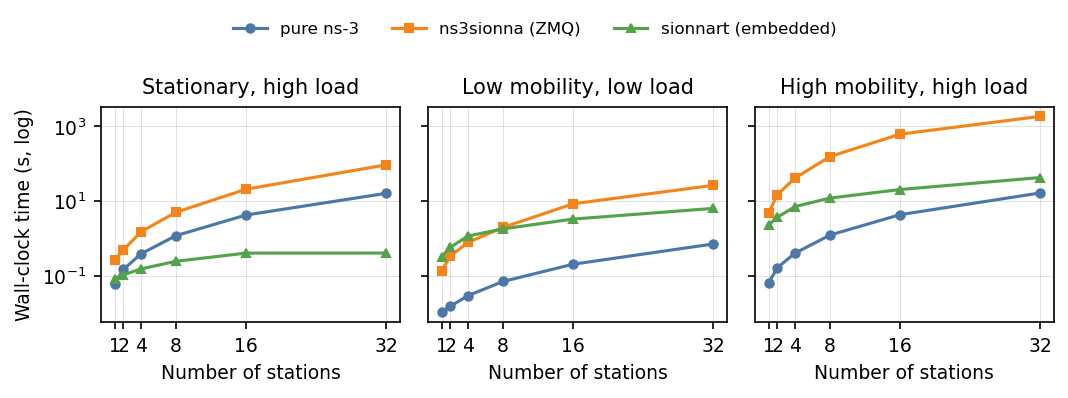
\includegraphics[width=\linewidth]{images/total-sim-time-scaling.png}
    \caption{Total simulation runtime of the three channel backends as the number of
        stations increases. The communication with external Sionna RT server via ZMQ in \texttt{ns3sionna} causes large overhead.
        The embedded \texttt{sionnart} backend avoids the round trip overhead, while the pure ns-3 baseline
        provides the analytical-channel lower bound.}
    \label{fig:total-sim-time-scaling}
\end{figure}

\begin{table}[t]
    \centering
    \caption{Total simulation runtime in seconds for representative station counts.}
    \label{tab:total-sim-time-scaling}
    \setlength{\tabcolsep}{5pt}
    \begin{tabular}{llrrrr}
        \hline
        Regime        & Backend   & $N=1$ & $N=4$  & $N=16$  & $N=32$   \\
        \hline
        Stationary    & pure ns-3 & 0.061 & 0.385  & 4.230   & 16.160   \\
        Stationary    & ns3sionna & 0.266 & 1.504  & 20.826  & 93.834   \\
        Stationary    & sionnart  & 0.082 & 0.152  & 0.403   & 0.404    \\
        \hline
        Low mobility  & pure ns-3 & 0.010 & 0.029  & 0.203   & 0.708    \\
        Low mobility  & ns3sionna & 0.137 & 0.778  & 8.453   & 26.439   \\
        Low mobility  & sionnart  & 0.320 & 1.153  & 3.292   & 6.370    \\
        \hline
        High mobility & pure ns-3 & 0.064 & 0.400  & 4.320   & 16.516   \\
        High mobility & ns3sionna & 4.821 & 41.312 & 622.365 & 1871.600 \\
        High mobility & sionnart  & 2.293 & 7.124  & 20.405  & 42.772   \\
        \hline
    \end{tabular}
\end{table}

The scaling behavior of time taken for simulation differs across different scenarios.
In the stationary scenario, the apparent advantage of \texttt{sionnart} over the \texttt{pure\_ns-3} baseline is an artefact of the cache (Section~\ref{subsec:cache-validity}), not evidence that ray-tracing is intrinsically faster than Friis evaluation.
Because no UE moves, the ray-tracer is invoked only once at $t=0$; all subsequent propagation queries are served from the cached channel snapshot while the analytical baseline still re-evaluates its loss model at every packet arrival.
This cache-driven effect produces an approximately $40\times$ wall-clock reduction at $N=32$, and would collapse to a significant overhead if mobility were introduced without the cache.
Even in this stationary scenario, \texttt{ns3sionna} backend is slower than both \texttt{pure\_ns-3} and \texttt{sionnart} backends due to the overhead of the communication between ns-3 and Sionna RT server.

In low-mobility, low-load scenario, the results show the opposite trade-off.
When the number of station counts ($N$) are low, \texttt{sionnart} is slower than \texttt{ns3sionna} because there are few propagation queries so that the cost of the query outweight the fixed cost of the embedded Python runtime and Sionna scene.
As $N$ grows, batching and cache reuse become more effective so that by the $N=32$ the performance of \texttt{sionnart} is 4.15 times faster than \texttt{ns3sionna}.
It remains 9 times slower than the \texttt{pure\_ns-3} baseline because the traffic load is low enough that stochastic propagation model remains cheap in term of computation.

The high-mobility, high-load scenario is the most important one because it is the most realistic scenario for the next generation wireless network.
In this scenario, \texttt{ns3sionna} scales poorly with the number of stations because each cache misses require copying data between processes, waiting for a request and response between two servers, and updating the Sionna side state.
The \texttt{sionnart} backend still have to pay the price of invoking the ray-tracer for each cache miss, but it avoid the overhead of inter-process communication and keeps the cache inside the same process.
As a result, the gap between \texttt{sionnart} and \texttt{ns3sionna}  grows monotonically from 2.1 times at $N=1$ to 43.8 times at $N=32$.


\subsubsection{Speedup Analysis}
\label{subsec:speedup-analysis}
Figire \ref{fig:speed-comparison} shows the runtime ratios.
The left panel shows $T_{\mathrm{ns3sionna}}/T_{\mathrm{sionnart}}$ and a larger value means that \texttt{sionnart} is faster than \texttt{ns3sionna}.
The right panel shows $T_{\mathrm{sionnart}}/T_{\mathrm{pure\ ns3}}$ and a value below one means that \texttt{sionnart} is faster than \texttt{pure\_ns-3} baseline.
The same results are show in Table \ref{tab:speed-comparison}.

\begin{figure}[t]
    \centering
    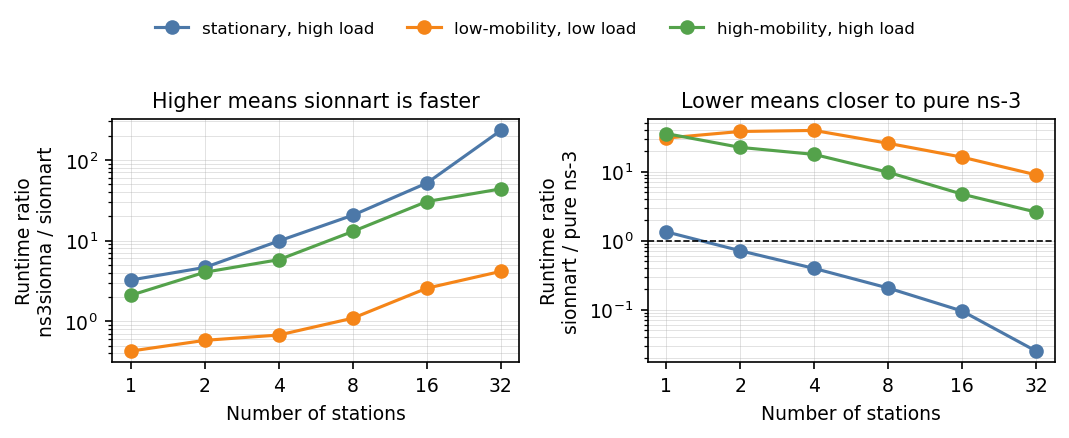
\includegraphics[width=\linewidth]{images/speed_comparison.png}
    \caption{The left graph shows the ratio of \texttt{ns3sionna} runtime to \texttt{sionnart} runtime.
        The right graph is the ratio of \texttt{sionnart} runtime to \texttt{pure\_ns-3} baseline runtime.}
    \label{fig:speed-comparison}
\end{figure}

According to these ratios, embedding Sionna RT using pybind11 helps to improve the performance of simulation.
In two server design, a cache miss must send data from ns-3 to a separate Python process and wait for the reply.
In the embedded design, ns-3, the cache, Sionna RT, all run inside the same process.
This removes much of the communication cost and the remaining cost is the actual ray-tracing, which is still needed when the experiment uses site-specific propagation.

\begin{table}[t]
    \centering
    \caption{Ratios at $N=32$. The first ratio is
    $T_{\mathrm{ns3sionna}}/T_{\mathrm{sionnart}}$; the second is
    $T_{\mathrm{sionnart}}/T_{\mathrm{pure\ ns3}}$.}
    \label{tab:speed-comparison}
    \setlength{\tabcolsep}{5pt}
    \begin{tabular}{lrr}
        \hline
        Scenario                 & Speedup over  & Cost relative \\
                                 & ns3sionna     & to pure ns-3  \\
        \hline
        Stationary, high load    & $232.3\times$ & $0.025\times$ \\
        Low mobility, low load   & $4.15\times$  & $9.00\times$  \\
        High mobility, high load & $43.8\times$  & $2.59\times$  \\
        \hline
    \end{tabular}
\end{table}

However, two server design is also have its own merits.
Having separate server for Sionna RT allows us to run the ray-tracing engine on a different machine, and it also allows us to run multiple ray-tracing engines in parallel.
But for our use case, we only need to run the ray-tracing engine on the same machine as ns-3.
So we choose the embedded design.

\subsubsection{GPU Footprint and Utilization}
\label{subsec:gpu-usage}

Figure \ref{fig:gpu-usage} shows the GPU memory footprint and processing core utilization for each scenario.
For \texttt{sionnart}, allocated memory is almost flat.
It is $337$ MiB for the smallest stationary scenario, about $465$-$469$ MiB for most scenarios, and $491$ MiB for the largest high-mobility scenario.
This is because most of the memory usage is due to the Sionna RT scene and increasing number of stations in the same scene, not the number of packets processed by ns-3.
By contrast, \texttt{ns3sionna} grows significantly in the high-mobility scenario.
The memory increases from $730$ MiB at $N=1$ to $7858$ MiB at $N=32$.

\begin{figure}[t]
    \centering
    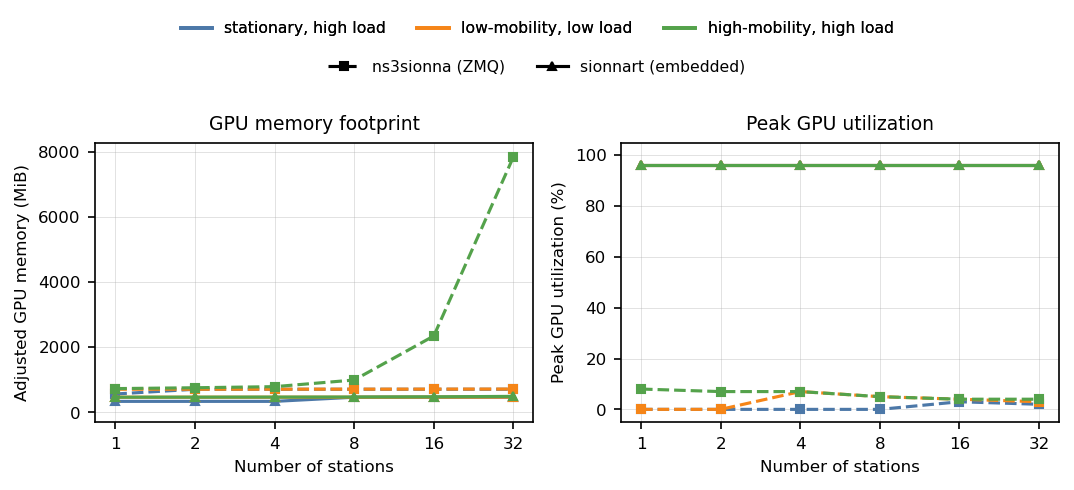
\includegraphics[width=\linewidth]{images/gpu_usage.png}
    \caption{Reported GPU memory footprint and peak utilization for the two
        Sionna-backed backends.}
    \label{fig:gpu-usage}
\end{figure}

The peak-utilization panel present the maximum observed value but not the average GPU load.
\texttt{sionnart} utilize upto $96\%$ at its peak for performing the channel calculations but the duration of running at peak is very short.
On the other hand, \texttt{ns3sionna} has lower peak utilization but the GPU is busy most of the time.

In summary, \texttt{sionnart} keeps a nearly fixed GPU memory footprint because the scene and others are reused across channel queries.
\texttt{ns3sionna} uses much more memory because it has to keep per-link ray-tracing state as the number of mobile links increases.
For \texttt{sionnart}, it utilize full potential of GPU and duration of running calculation is very short while the \texttt{ns3sionna} is busy most of the time with lower peak utilization.


\section{Application Case Study: massive MIMO 5G Evaluation}
\label{sec:exp2-nr-energy}

Having successfully verified the computational efficiency and scalability of our embedded simulation framework, we now demonstrate its practical utility through a realistic 3GPP~NR deployment case study \cite{5glena,tr38901}.
This section showcases how the integrated Sionna~RT backend allows researchers to evaluate end-to-end 5G massive MIMO networks. We assess critical application-level KPIs (throughput, packet loss, delay, jitter), propagation-level KPIs (path loss, path delay, CQI, MCS), and overall energy consumption. To provide a comprehensive evaluation, we simulate three distinct radio environments—free space, urban macro, and urban micro—using gNB antenna array sizes ranging from $2\times2$ to $8\times8$, under varying traffic loads.

\subsection{Experiment Configuration}
\label{subsec:exp2-setup}

In each simulation run, one gNB and 20 UEs are used.
The UE count is fixed to 20 to keep per-step GPU memory and simulation wall-clock time within practical bounds on the evaluation hardware; scaling to denser deployments is outside the scope of this work.
The gNB antenna array is varied over $2\times2$, $4\times4$, and $8\times8$; each UE uses a fixed $2\times2$ array.
The simulations are tested in three different radio environments:
\begin{itemize}
    \item \textbf{free space}: $2$ GHz carrier, $35$ m gNB height, and UE
          distances from $50$ m to $1000$ m;
    \item \textbf{urban macro}: $3.5$ GHz carrier, $25$ m gNB height, and UE
          distances from $35$ m to $500$ m;
    \item \textbf{urban micro}: $28$ GHz carrier, $10$ m gNB height, and UE
          distances from $10$ m to $200$ m.
\end{itemize}
The carrier frequencies, antenna heights, and UE distance ranges are aligned with the 3GPP TR 38.901 reference deployment configurations \cite{tr38901}.
The 2~GHz carrier for the free-space baseline corresponds to the FR1 sub-3~GHz band; the 3.5~GHz urban macro carrier matches the primary 5G~NR band (n78, FR1); and the 28~GHz urban micro carrier represents the FR2 mmWave band (n257/n261).
The gNB heights of 25~m (urban macro) and 10~m (urban micro) follow the TR~38.901 UMa and UMi reference values respectively, while the 35~m free-space height is consistent with rural macro conventions.
The UE distance ranges are chosen to cover the minimum coupling distance and approximate cell radius defined for each scenario in TR~38.901 Table~7.2-1.
The single-cell, 20-UE configuration is consistent with the single-sector system-level evaluation methodology of TR~38.901 Table~A.1.
The free-space scenario is the baseline, the urban macro scenario represents a sub-6~GHz deployment, and the urban micro scenario represents the most demanding physical setting as it combines a mmWave carrier with geometry-sensitive, short-range links.
The 3D visualizations of these three environments are shown in Figure~\ref{fig:scenarios}.

\begin{figure}[t]
    \centering
    \subfloat[Free space.]{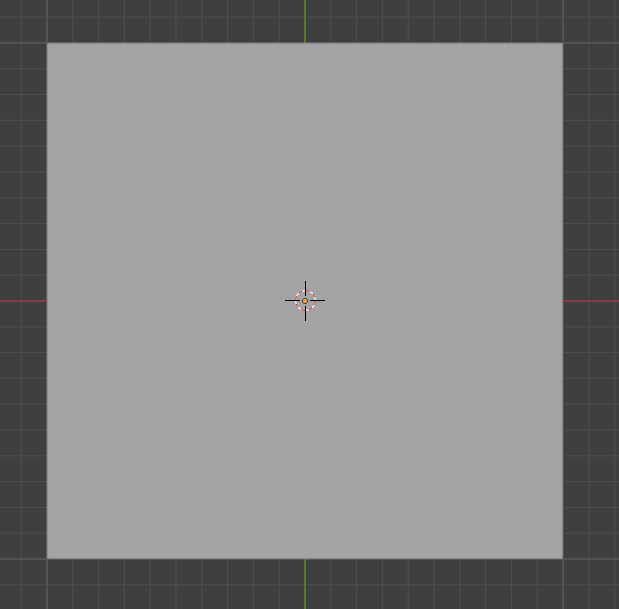
\includegraphics[width=0.32\linewidth]{images/free_space.png}\label{fig:scenario_free_space}}
    \hfill
    \subfloat[Urban macro.]{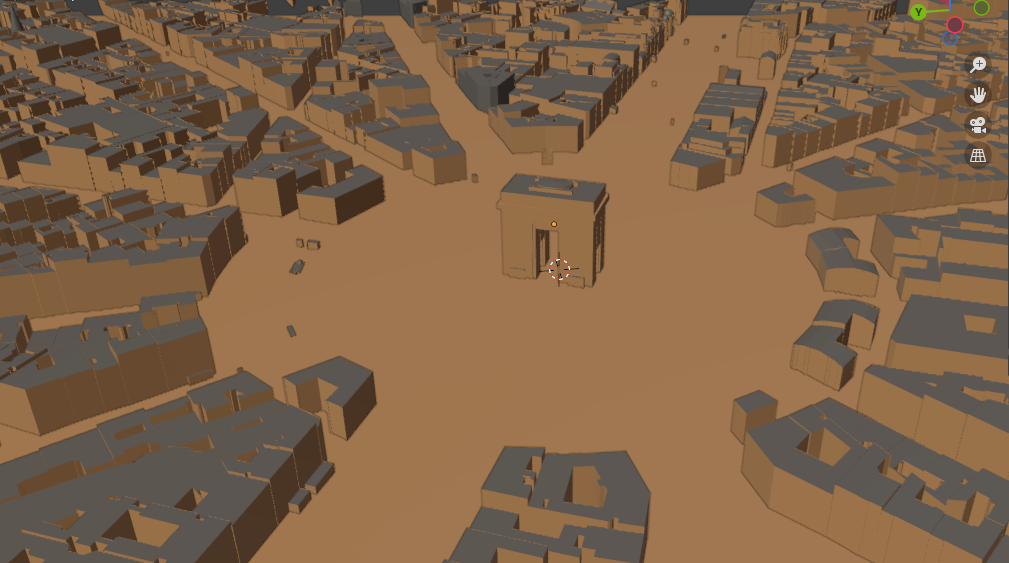
\includegraphics[width=0.32\linewidth]{images/urban_macro.png}\label{fig:scenario_urban_macro}}
    \hfill
    \subfloat[Urban micro.]{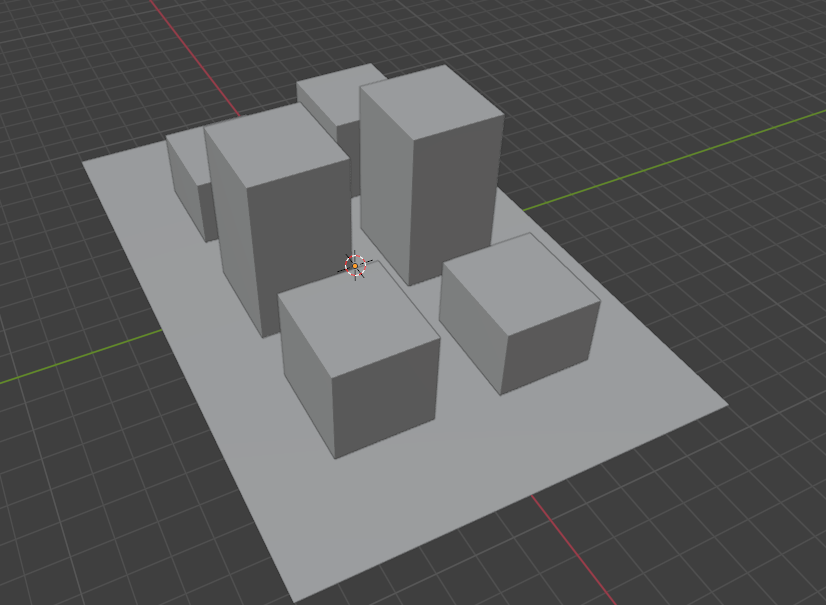
\includegraphics[width=0.32\linewidth]{images/urban_micro.png}\label{fig:scenario_urban_micro}}
    \caption{The three simulated radio environments.}
    \label{fig:scenarios}
\end{figure}

For scheduling UEs, a TDMA proportional fair scheduler, and full-buffer TDD slots are used.
On top of the realistic wireless channel model, different applications with different traffic loads are tested.
The traffic profile includes video, voice over IP (VoIP), social media, gaming, and FTP.
The per-application UE distribution — 12 (60\%), 2 (10\%), 2 (10\%), 1 (5\%), and 3 (15\%) for video, VoIP, social media, gaming, and FTP respectively — follows the traffic mix proportions reported in \cite{ericsson_mobility}, and is applied identically for both DL and UL.
The data rate for each application according to load levels are summarized in Table \ref{tab:exp2-offered-load}.

\begin{table*}[t]
    \centering
    \caption{Application data rate by application and load.}
    \label{tab:exp2-offered-load}
    \begin{tabular}{lrrrrrrr}
        \hline
        Application                & Flows                    & \multicolumn{2}{c}{Low} &
        \multicolumn{2}{c}{Medium} & \multicolumn{2}{c}{High}                                                                                       \\
        \cline{3-8}
                                   &                          & DL (Mbps)               & UL (Mbps) & DL (Mbps) & UL (Mbps) & DL (Mbps) & UL (Mbps) \\
        \hline
        Video                      & 12 DL / 12 UL            & 24.000                  & 0.300     & 96.000    & 1.200     & 300.000   & 3.750     \\
        VoIP                       & 2 DL / 2 UL              & 0.128                   & 0.032     & 0.256     & 0.064     & 2.000     & 0.500     \\
        Social                     & 2 DL / 2 UL              & 1.000                   & 0.050     & 10.000    & 0.500     & 40.000    & 2.000     \\
        Gaming                     & 1 DL / 1 UL              & 0.100                   & 0.025     & 1.000     & 0.250     & 10.000    & 2.500     \\
        FTP                        & 3 DL / 3 UL              & 3.000                   & 0.150     & 30.000    & 1.500     & 150.000   & 7.500     \\
        \hline
        Total                      & 20 DL / 20 UL            & 28.228                  & 0.557     & 137.256   & 3.514     & 502.000   & 16.250    \\
        \hline
    \end{tabular}
\end{table*}


\subsection{Free-Space Scenario}
\label{subsec:exp2-free-space}

The free-space scenario serves as the baseline because it has no building blockage; distance is the sole large-scale factor.
UEs are distributed up to $1000$~m from the gNB, so the scenario combines strong near-field links with very weak cell-edge links.

\subsubsection{Application-related Metrics}
\label{subsubsec:exp2-free-space-flow}

Figure~\ref{fig:exp2-free-space-flow} shows per-application throughput, packet loss, delay, and jitter for both directions and all antenna configurations.
The stochastic ns-3 model outperforms Sionna~RT in average downlink throughput: at $8\times8$, ns-3 delivers $4.85$~Mbit/s ($21.6\%$ loss) versus $3.77$~Mbit/s ($26.6\%$ loss) for Sionna~RT, with the same ordering at $2\times2$.
The gap reflects the large cell radius: UEs at the cell edge experience greater path loss under ray tracing than the stochastic model predicts.
Array scaling yields only marginal throughput gain in both simulators because the bottleneck is cell-edge path loss, not beamforming resolution.

\begin{figure*}[t]
    \centering
    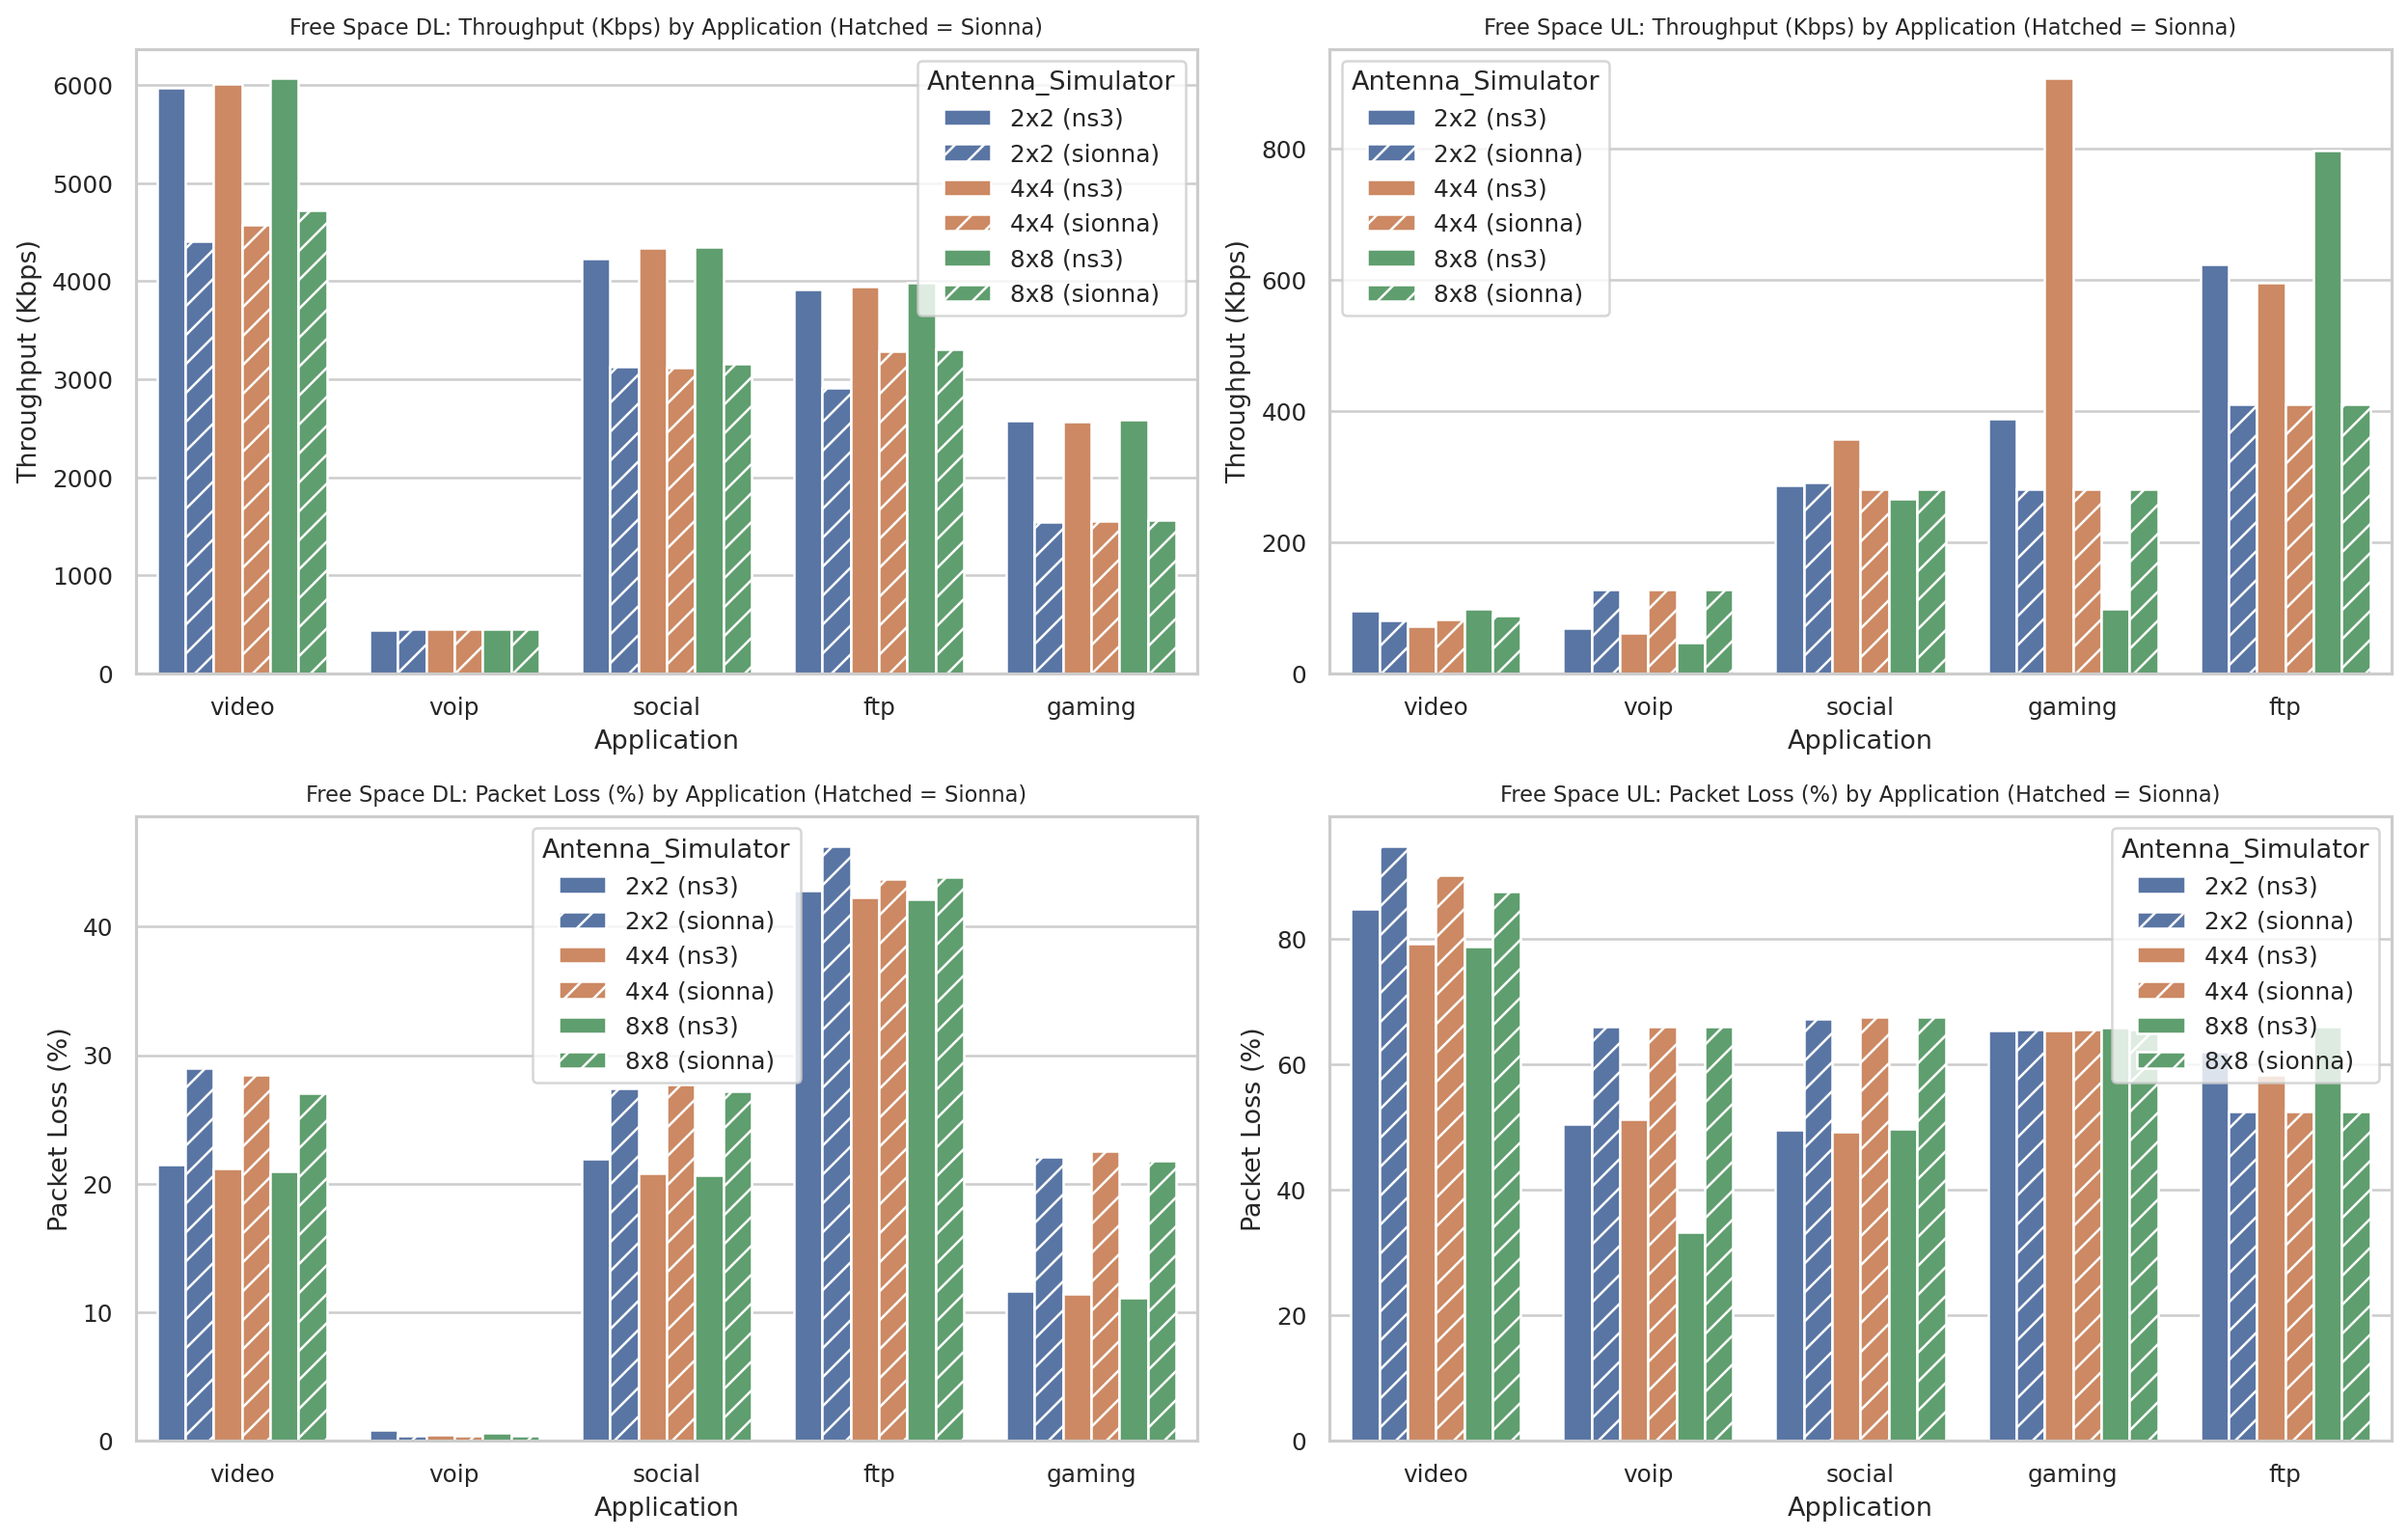
\includegraphics[width=\textwidth]{images/free_space_flow_metrics.png}
    \caption{Free-space application-level throughput and packet loss by application, direction, and gNB array size. Solid bars: ns-3; hatched bars: Sionna~RT.}
    \label{fig:exp2-free-space-flow}
\end{figure*}

\subsubsection{Propagation-related Metrics}
\label{subsubsec:exp2-free-space-propagation}

Average path loss is $94.2$~dB and estimated receive power is $-48.2$~dBm for both channel models (Fig.~\ref{fig:exp2-channel-quality}).
The ns-3 model reports a mean path delay of $3059$~ns while Sionna~RT reports $2237$~ns; both are consistent with radio path lengths of hundreds of metres.
CQI and MCS improve monotonically with array size in both simulators.
At $8\times8$, ns-3 reaches mean CQI~$15$ and MCS~$27$; Sionna~RT reaches CQI~$14.79$ and MCS~$26.59$.
The gap is small in free space because most links are near-line-of-sight; array gain raises channel quality but cannot overcome path loss for the most remote UEs.

\subsubsection{Energy Consumption-related Metrics}
\label{subsubsec:exp2-free-space-energy}

gNB power consumption increases with array size in both simulators (Fig.~\ref{fig:exp2-gnb-power}).
In ns-3, the gNB consumes $31.16$~W ($2\times2$), $64.58$~W ($4\times4$), and $199.39$~W ($8\times8$); Sionna~RT reports $30.08$~W, $59.08$~W, and $173.50$~W respectively.
UE power is similar across all configurations because the UE array is fixed at $2\times2$.
The throughput-per-watt trade-off is poor for larger arrays in this scenario: $8\times8$ consumes roughly six times the gNB power of $2\times2$ while delivering only marginal throughput gains.
Array gain cannot offset the scheduling pressure of serving many long-distance UEs under high traffic load.


\subsection{Urban Macro Scenario}
\label{subsec:exp2-urban-macro}

The urban macro scenarios is based on the Charles de Gaulle Etoile in Paris, which is a dense urban environment with tall buildings and many obstacles.
The gNB is placed at the top of the Arc de Triomphe at a height of $25$ m and UEs are distributed in a circle of radius $500$ m around the gNB.
The antennas are configured to use the $3.5$ GHz carrier frequency, which is in the sub 6-Hz range.
This scenario is one of the challenging scenario for 6G network deployments due to the high density of buildings and obstacles.

\subsubsection{Application-related Metrics}
\label{subsubsec:exp2-urban-macro-flow}

Figure \ref{fig:exp2-urban-macro-flow} illustrates the application-related metrics for the urban macro scenario, comparing ns-3 (solid bars) and Sionna RT (hatched bars) across various antenna configurations.
Among the traffic types, data-intensive applications such as FTP and video streaming achieve the highest throughput in both simulators.
For FTP, ns-3 outperforms Sionna RT at the $2 \times 2$ configuration where ns-3 achieve roughly $16.8$ Mbps whereas Sionna RT achieve $15.2$ Mbps.
But as the gNB array size increase to $4 \times 4$ and $8 \times 8$, Sionna RT perform better than ns-3 and achieve nearly $19.5$ Mbps whereas ns-3 achieve $18.5$ Mbps.
The statistical ns-3 approach performs well generally but Sionna RT approach performs better at larger array size as it can better leverage massive MIMO spatial multiplexing by capturing multipath components such as reflections and diffractions from the buildings and environment.
In contrast, for video streaming application, ns-3 consistently achieve higher than Sionna RT across all antenna configurations.

For Sionna RT, higher packet loss for video traffic is observed in downlink which values are $9.5\%$, $7.6\%$ and $4.6\%$ respectively for $2 \times 2$, $4 \times 4$ and $8 \times 8$ antenna configurations.
Ns-3 performs better than Sionna RT for video traffic and for FTP traffic under $2 \times 2$ configuration, however, Sionna RT outperforms ns-3 for FTP traffic under $4 \times 4$ and $8 \times 8$ configurations.
Overall, increasing the antenna array size significantly reduce packet loss for most of the applications in both simulators.
In the uplink, the packet loss for all most all of the applications are very high for both simulators, ranging from $15\%$ for VoIP to nearly $100\%$ for gaming and social applications in Sionna RT.
This reflects the impact of harsh environment conditions on the constrained transmission power of UEs which struggles to overcome severe blockages, resulting in poor uplink condition.
Interestingly, Sionna RT still achieve higher throughput than ns-3 for gaming and FTP traffic in uplink eventhough Sionna RT observe higher packet loss than ns-3 for both applications.

Packet delay and jitter metrics further align with these observations.
Downlink delay is worst for video and FTP traffic where Sionna RT achieve $295$ ms, $220$ms, and $175$ ms for FTP and $220$ ms, $145$ ms, and $65$ ms for video, respectively for $2\times2, 4\times4, 8\times8$ antenna configurations.
Ns-3 also observes high delay for video and FTP traffic in downlink as well, however, it is lower than Sionna RT.
The reason Sionna RT experience higher delay is because the detailed multipath components captured by ray-tracing introduce longer propagation paths and varying signal arrival times, increasing the queuing delay.
Jitter remains relatively low in both simulators for all the applications but ns-3 occasionally reports high spike for application like FTP and gaming.

\begin{figure*}[t]
    \centering
    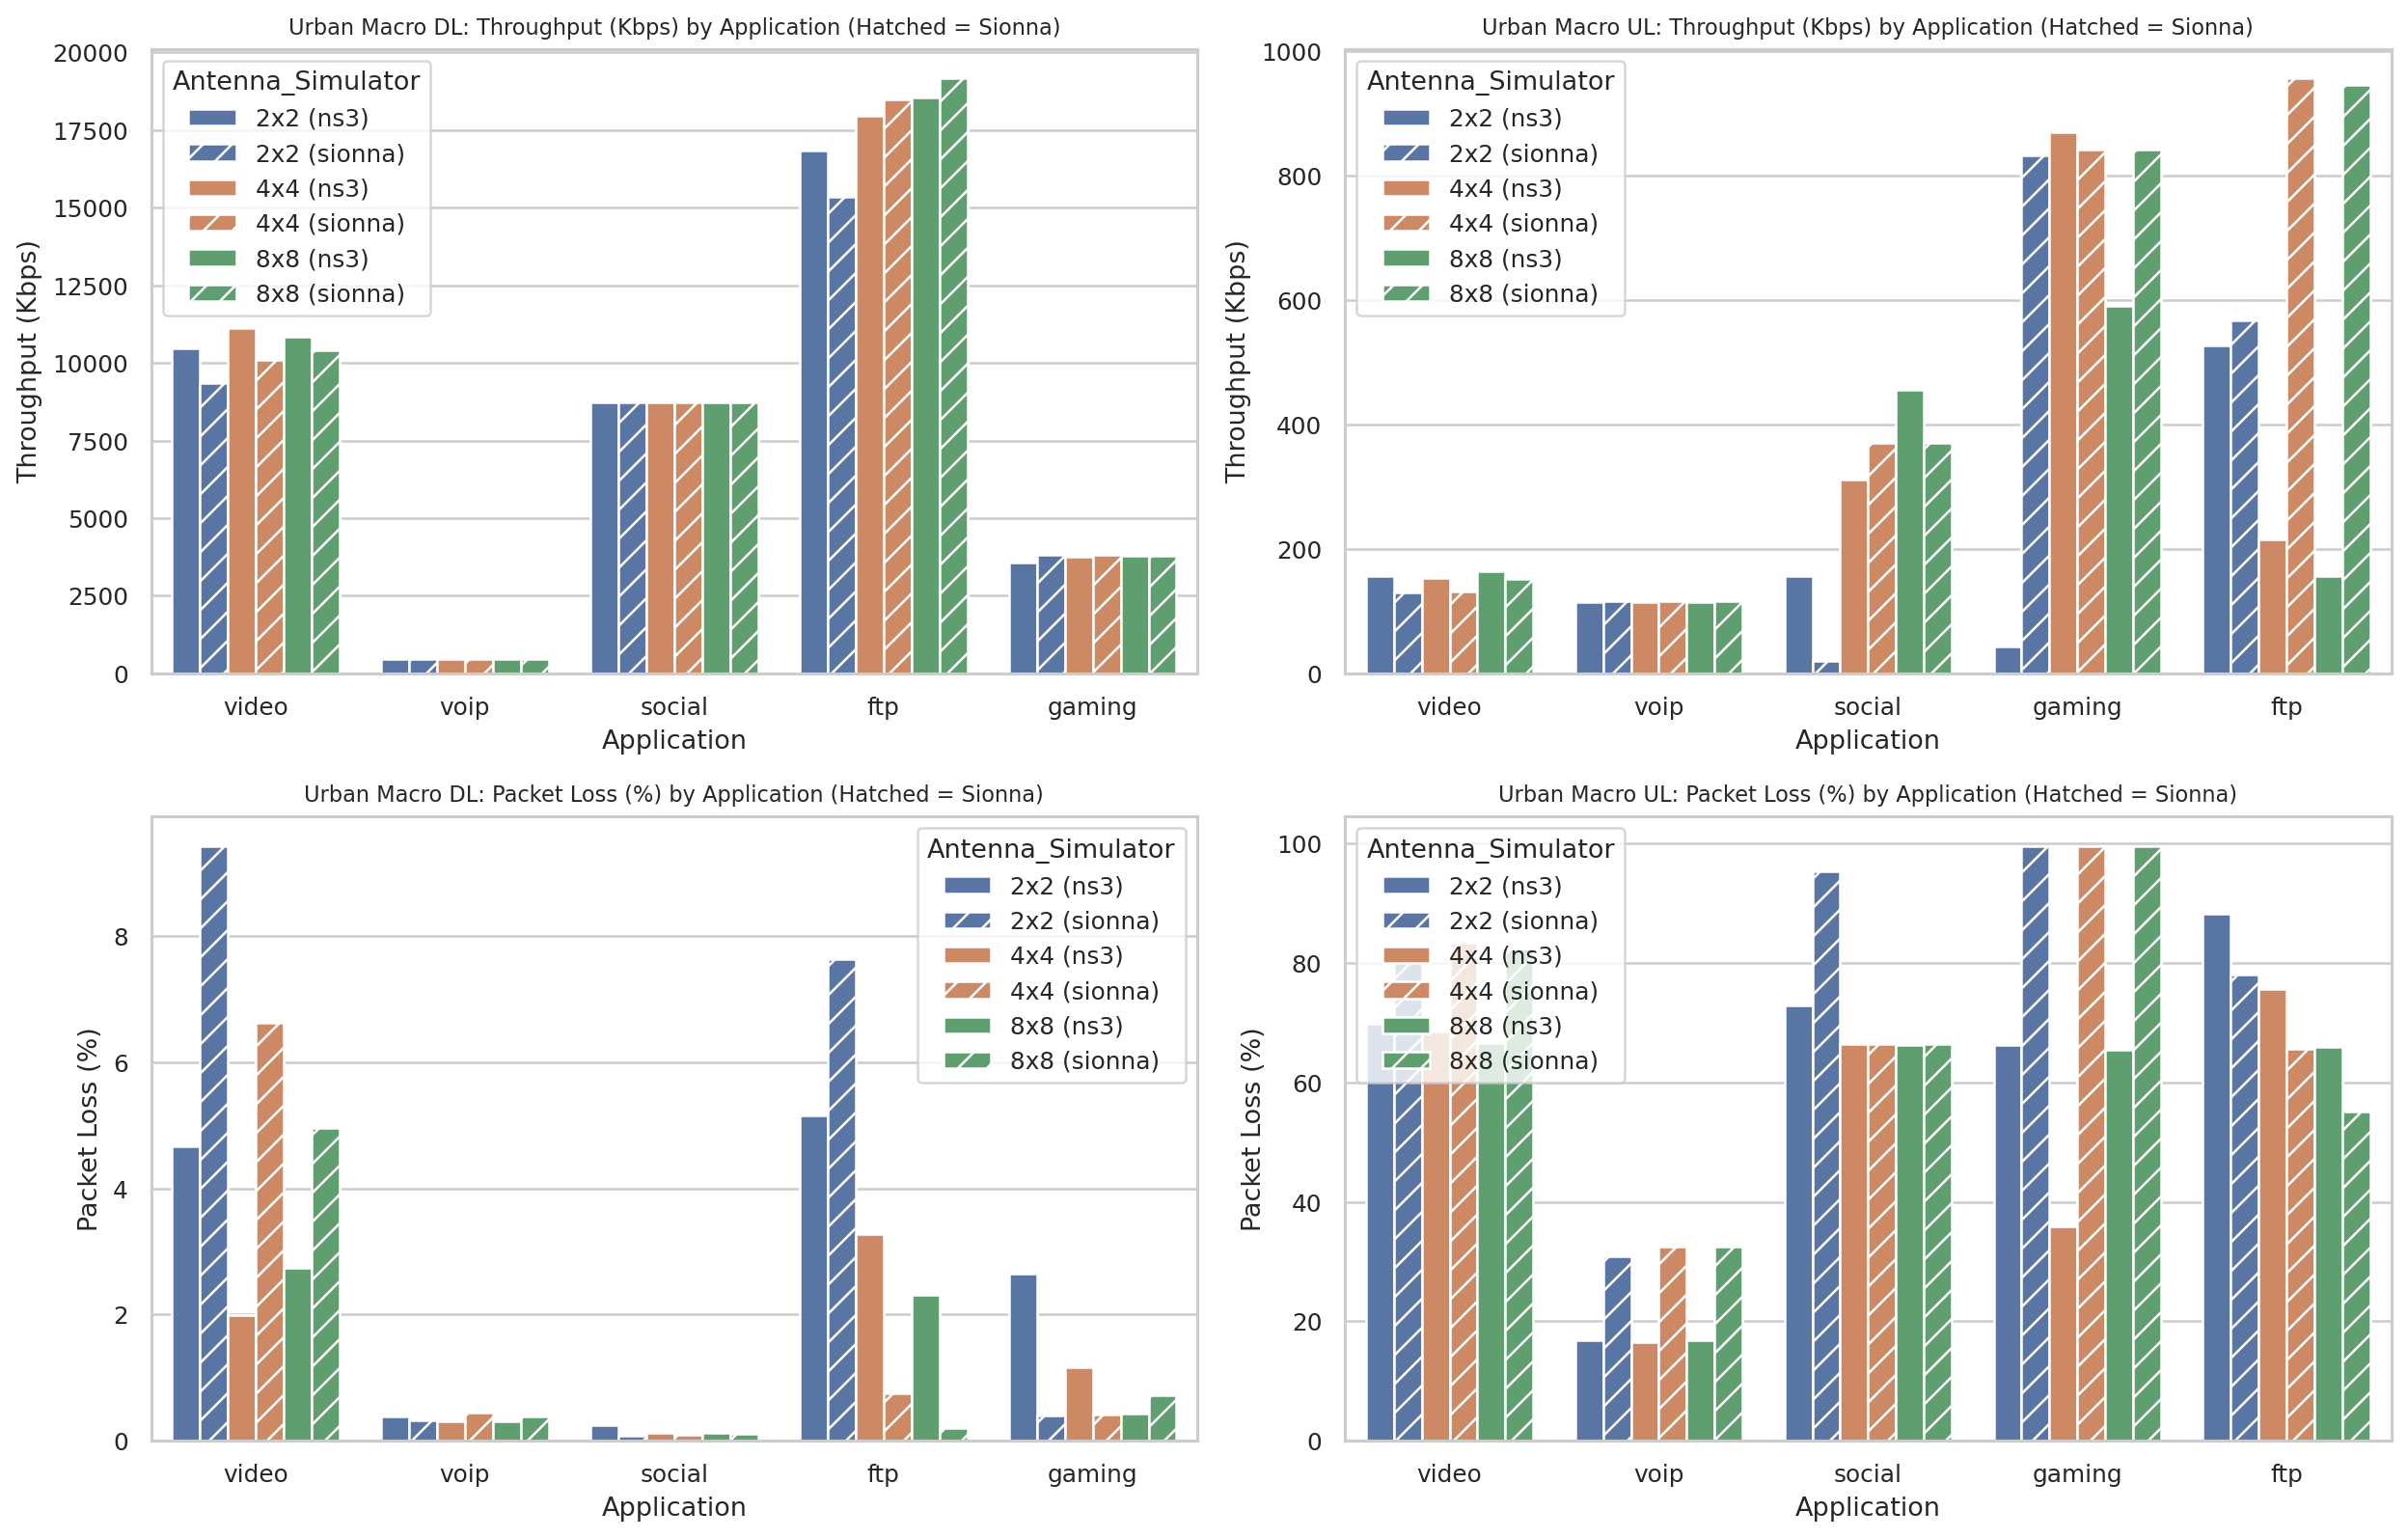
\includegraphics[width=\textwidth]{images/urban_macro_flow_metrics.png}
    \caption{Urban macro Application-related metrics by traffic type, direction, and
        gNB array size.}
    \label{fig:exp2-urban-macro-flow}
\end{figure*}


\subsubsection{Propagation-related Metrics}
\label{subsubsec:exp2-urban-macro-propagation}

The propagation-related results are presented in Figure \ref{fig:exp2-urban-macro-propagation}.
Path loss and received power remain consistent across all antenna size in both simulators at roughly $83.5$ dB and $-37.5$ dBm respectively.
Both ns-3 and Sionna RT achieve nearly identical values for propagation related metrics but differences can only be observed in path delay, CQI and MCS.
Ns-3 estimate a path delay of approximately $220$ ns while Sionna RT estimate higher delay around $360$ ns across all antenna configurations.
Higher delay in Sionna RT was due to taking into consideration for multipath components.

Similarly, lower CQI and MCS values are observed in Sionna RT than ns-3 for all antenna configurations.
For instance, in the $2 \times 2$ configuration, Sionna RT reports an average CQI of $9.5$ and MCS of $16.5$ while ns-3 estimates a CQI of $10.5$ and MCS of $17.5$.
Nevertheless, increasing gNB array size from $2 \times 2$ to $8 \times 8$ improves CQI and MCS in both simulators.
For example,  Sionna RT reports an average CQI of $10$ and MCS of $17$ at $8\times8$ configuration while ns-3 estimates a CQI of $11$ and MCS of $18$.
Improving CQI and MCS according to gNB array size validate that increasing the array size enhances beamforming capabilities and effectively reduces impact of environment and improves overall link quality.


\begin{figure*}[t]
    \centering
    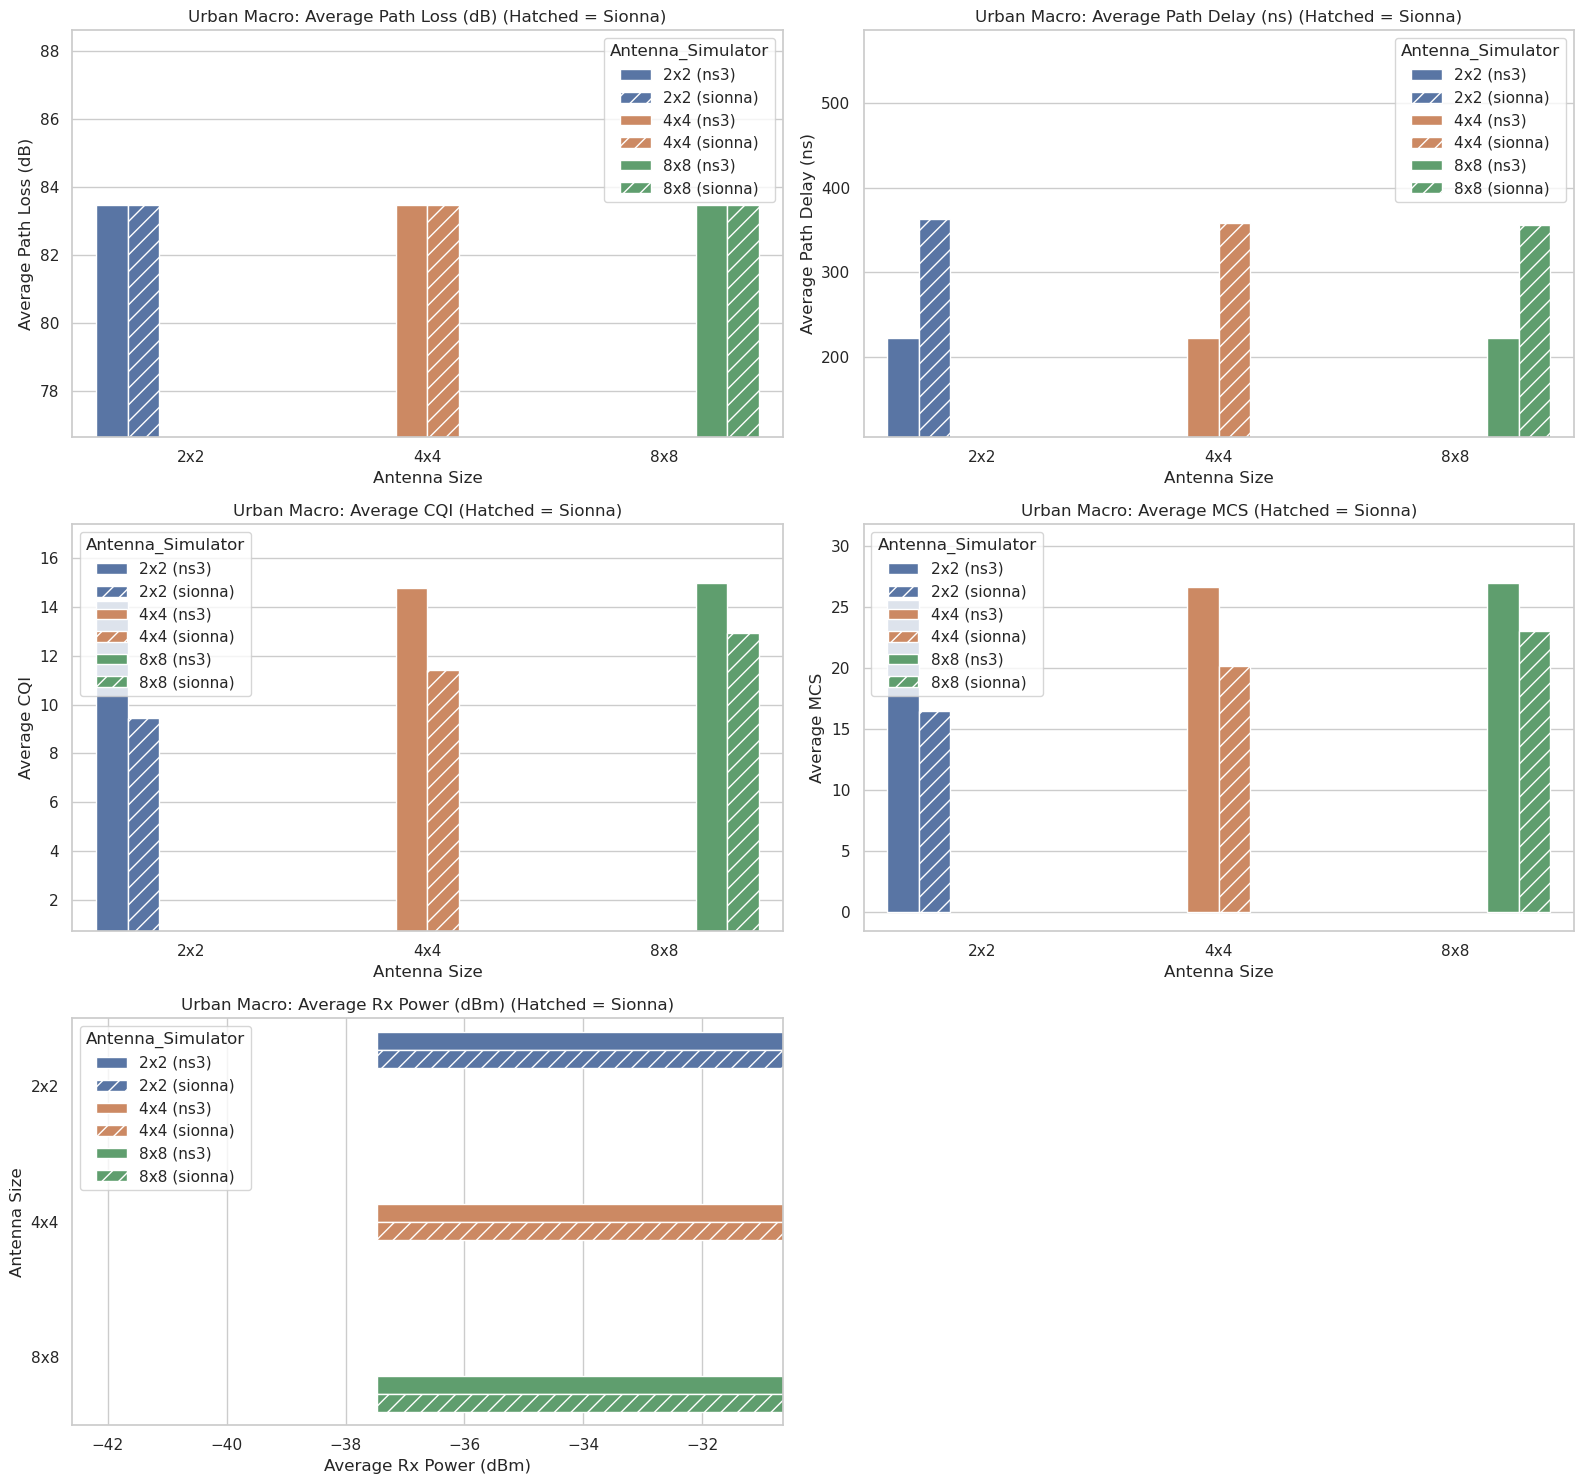
\includegraphics[width=\textwidth]{images/urban_macro_propagation_metrics.png}
    \caption{Urban macro propagation-related metrics by channel mode and gNB array
        size.}
    \label{fig:exp2-urban-macro-propagation}
\end{figure*}


\subsubsection{Energy Consumption-related Metrics}
\label{subsubsec:exp2-urban-macro-energy}\

In Figure \ref{fig:exp2-urban-macro-energy}, the energy consumptions of gNB and UEs by array size, and traffic load are presented.
The power consumption of gNB scales accordingly with both antenna array size and traffic load and both simulators show similar scaling trends.
For instance, both ns-3 and Sionna RT reports approximately $25$ W, $40$ W and $100$ W for $2\times2, 4\times4, 8\times8$ array configurations under low traffic load.
However, Sionna RT reports slightly higher power consumption than ns-3 for all antenna configurations.
The reason is link to lower CQI and MCS values estimated by Sionna RT, which alters resource block allocations and transmission durations compared to ns-3.
These results show that increasing gNB array size improve performance but at the cost of significantly higher energy consumption.

The power consumption of UE remains relatively stable for all antenna configurations in both simulators but scale noticeably with traffic load.
The UE power consumption increases from approximately $0.058$ W at low load to nearly $0.095$ W at high load.
Both simulator observe nearly identical UE power consumption across all configurations but Sionna RT consumes slightly higher energy than ns-3.
This is because UE are constrained to $2 \times 2$ antenna configuration in this experiment.

\begin{figure*}[t]
    \centering
    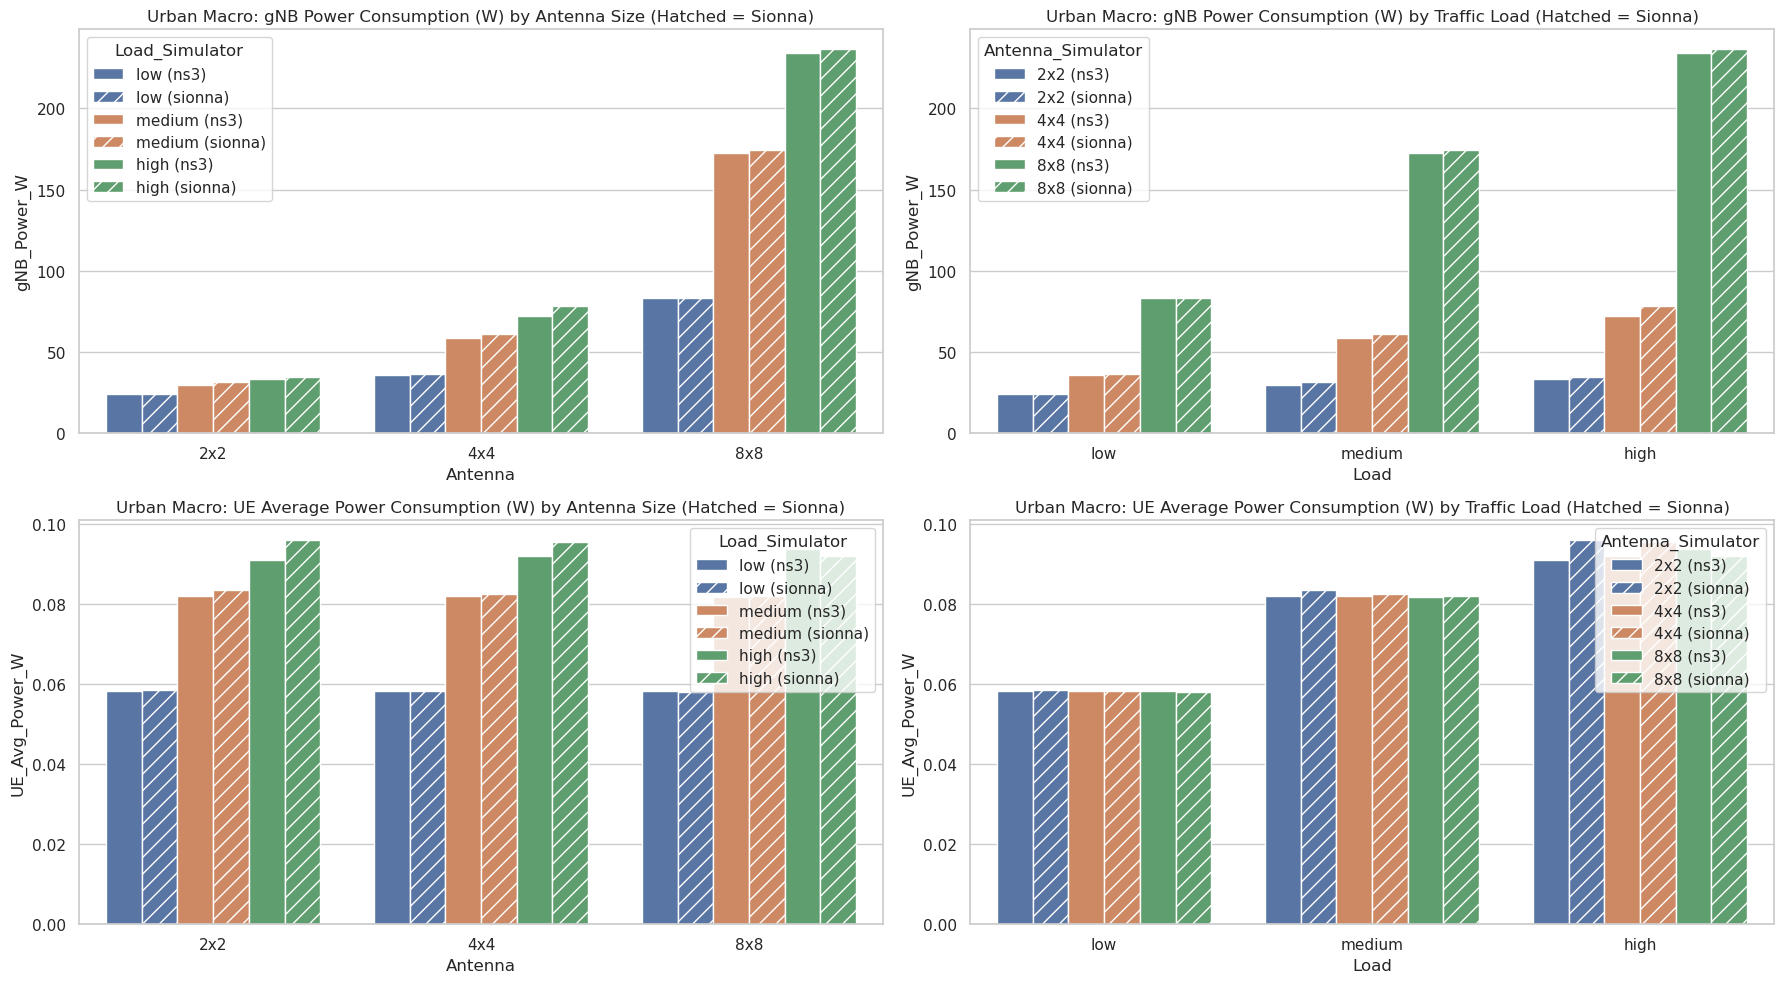
\includegraphics[width=\textwidth]{images/urban_macro_power_consumption.png}
    \caption{Urban macro energy consumptions of gNB and UEs by array size, and
        traffic load.}
    \label{fig:exp2-urban-macro-energy}
\end{figure*}

\subsection{Urban Micro Scenario}
\label{subsec:exp2-urban-micro}

The urban micro scenario is designed to simulate the dense street-level environment where gNB is deployed at lower elevation of $10$ m, typically below the surrounding rooftops.
In this scenario, the likelihood of non-line-of-sight (NLOS) conditions and strong multipath effects due to scattering from nearby buildings and street furniture is higher compared to the macro scenario.
The complex propagation environment presents unique challenges for establishing reliable links, especially for high-throughput applications.

\subsubsection{Application-related Metrics}
\label{subsubsec:exp2-urban-micro-flow}

Figure \ref{fig:exp2-urban-micro-flow} illustrates the application-level flow metrics for the urban scenario.
A comparative analysis between the statistical ns-3 model (solid bars) and the ray-tracing Sionna model (hatched bars) reveals substantial differences in how each simulator resolves the complex 3D urban environment.
In terms of downlink throughput, Sionna RT consistently achieve higher throughput for data-intensive applications such as FTP and gaming compared to ns-3.
For example, in Sionna RT, FTP throughput reach nearly $20$ Mbps with $4 \times 4$ and $8 \times 8$ gNB antenna array sizes while ns-3 reach around $15$ Mbps.
This mean that Sionna RT approach capture multipath components (reflections and diffractions) from urban structures which lead to higher downlink throughput than ns-3 approach when MIMO spatial multiplexing is leveraged.
Consistent with the trends observed in the macro scenario (Section~\ref{subsec:exp2-urban-macro}), scaling from $2\times2$ to $8\times8$ clearly improves throughput in both simulators.

The packet loss metrics further emphasize the environmental impact.
In downlink, ns-3 get high packet loss for FTP and gaming, nearly $30\%$ in $2\times2$ configuration, while Sionna RT get lower loss rate for these applications.
In contrast, Sionna~RT reports higher loss for video traffic at $2\times2$.
In both cases, scaling to $8\times8$ reduces downlink packet loss to near-zero for most applications, demonstrating how massive MIMO overcomes urban blockage.
The uplink remains severely loss-limited ($60\%$–$90\%$ in both simulators), reflecting the fundamental constraint that UE transmit power is insufficient to overcome dense urban obstacles without a reciprocal beamforming advantage at the receiver.

Packet delay and jitter metrics also align with the previous observations.
Downlink delay is worst under $2 \times 2$ array configuration, with ns-3 experiencing extreme spikes for FTP $>350$ ms and Sionna RT showing elevated delays for video and social traffic.
The multipath components captured by ray-tracing can introduce variable signal arrival times, occasionally increasing delay and jitter for continuous streams in Sionna RT.
However, as the gNB array scales to $8 \times 8$, both delay and jitter drop significantly which confirms that massive MIMO is essential for meeting the strict latency and reliability requirements of 6G applications in dense urban areas.


\begin{figure*}[t]
    \centering
    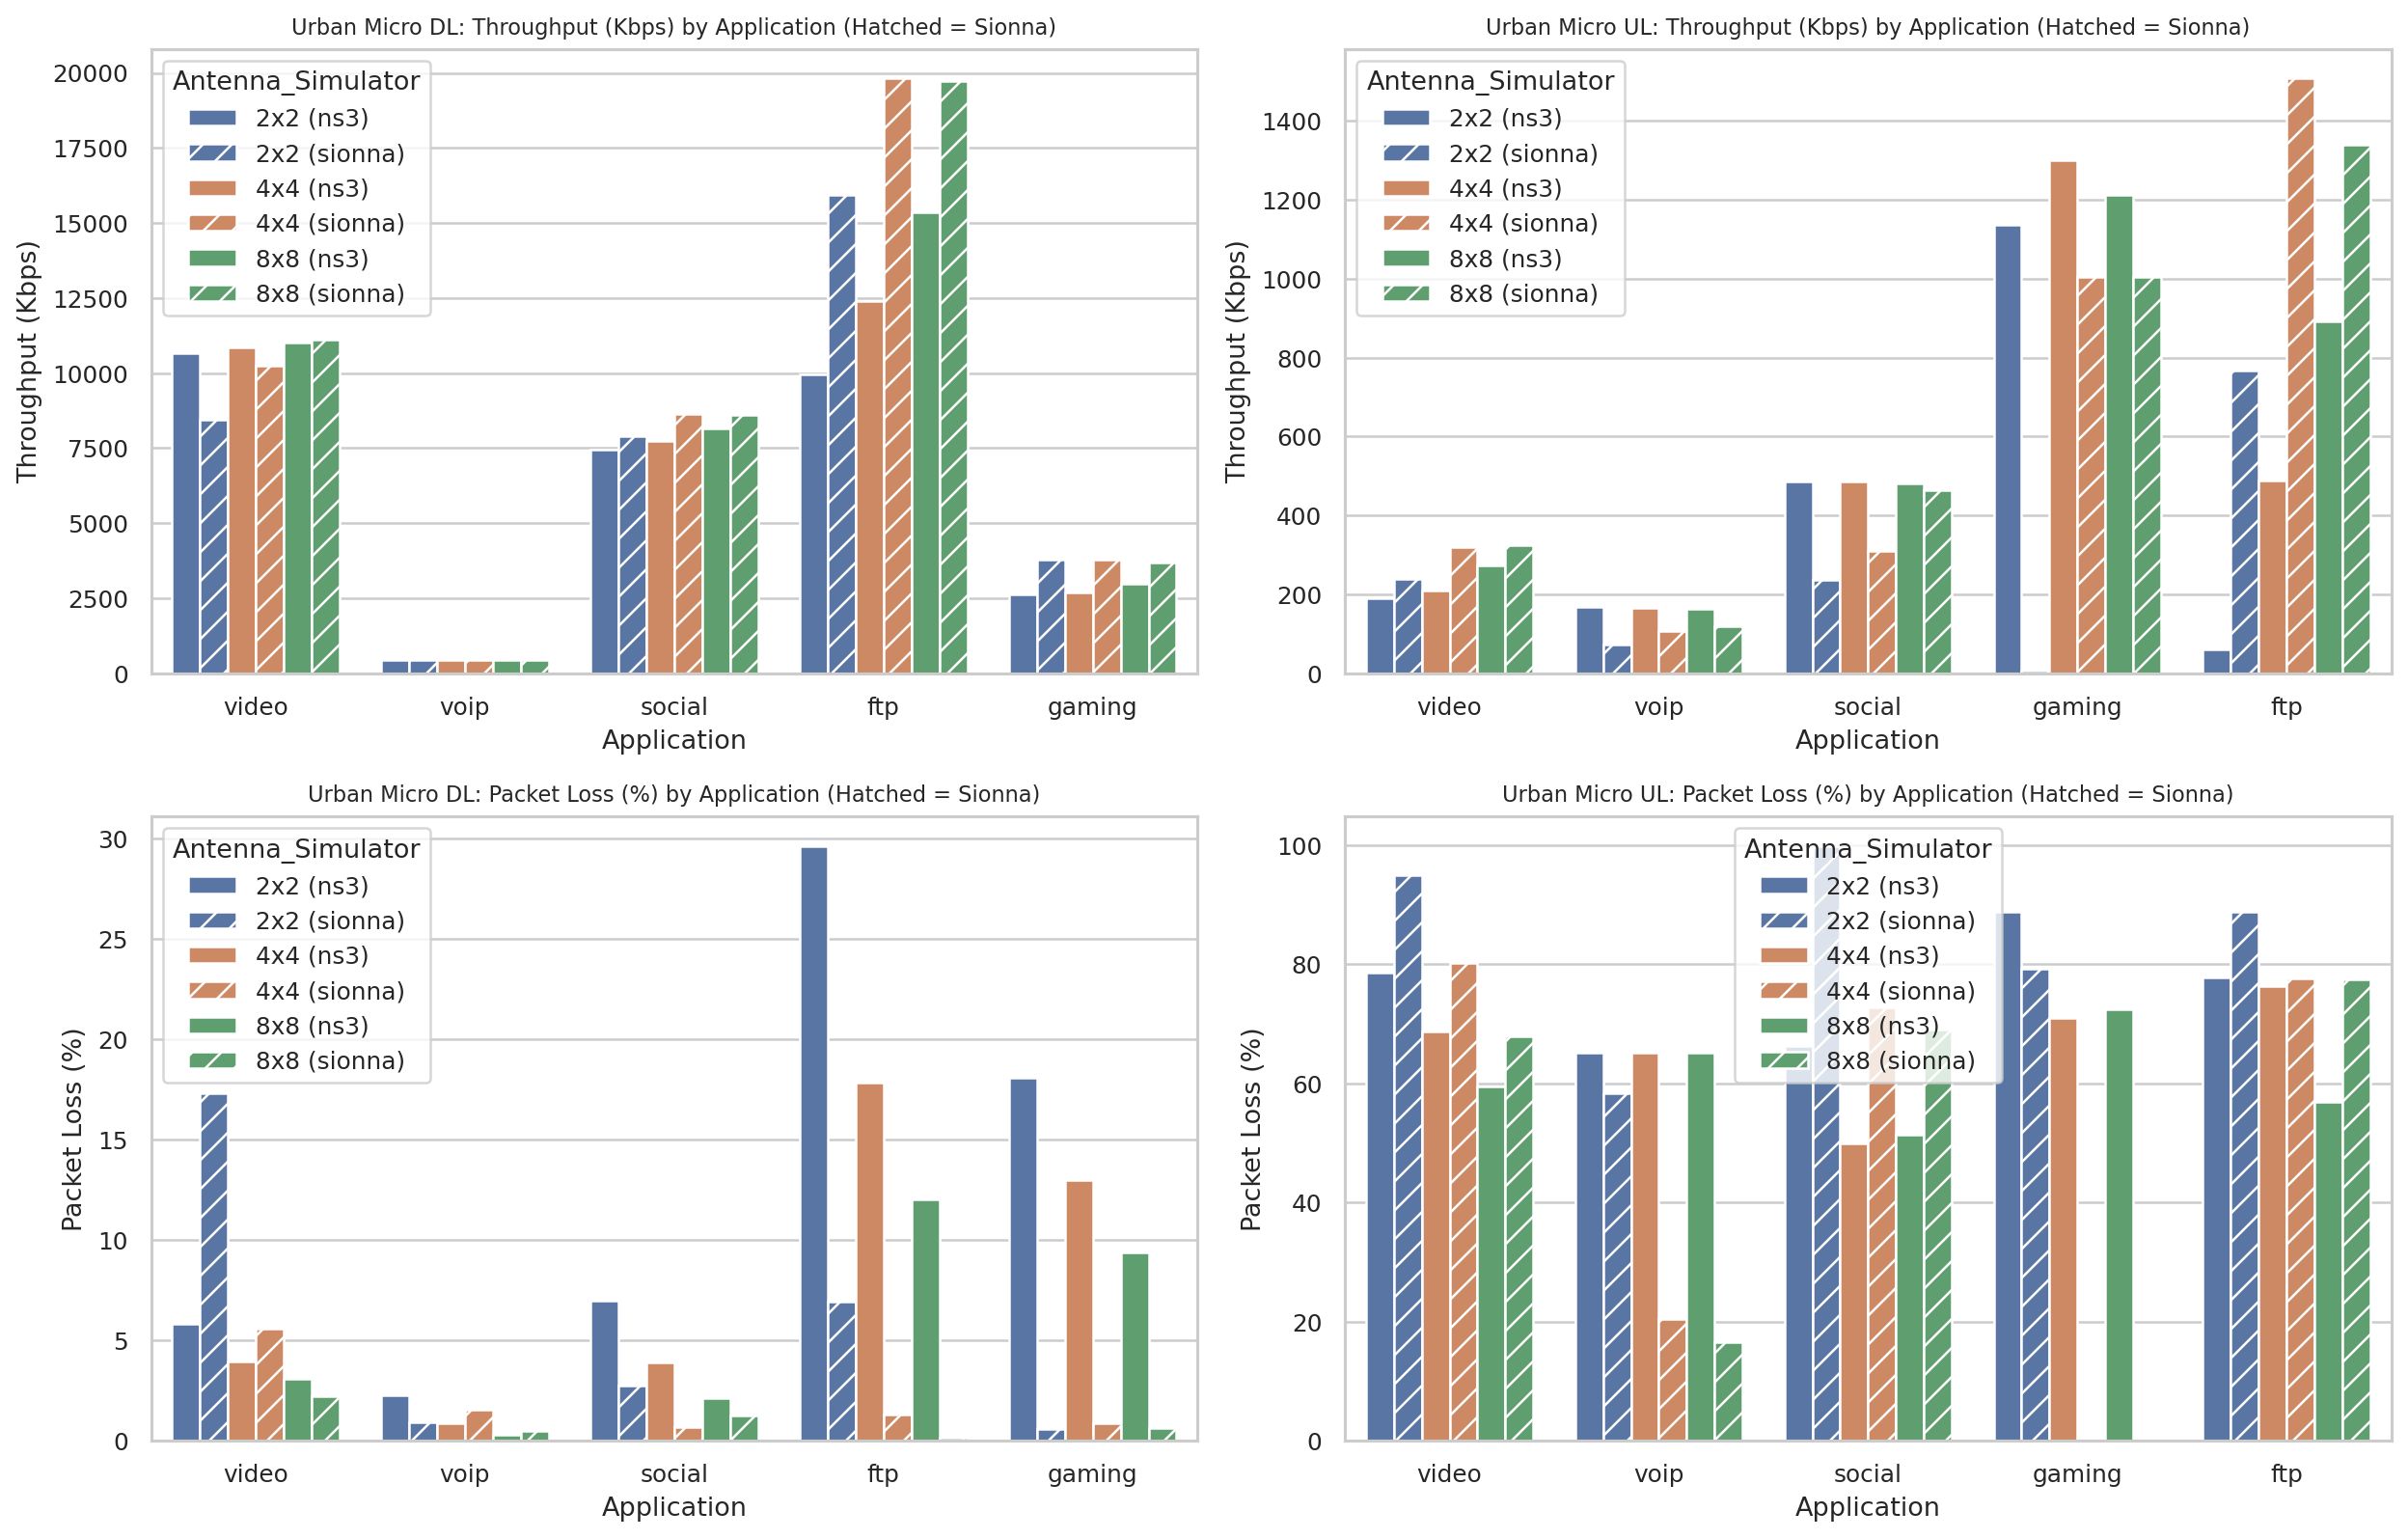
\includegraphics[width=\textwidth]{images/urban_micro_flow_metrics.png}
    \caption{Urban micro Application-related metrics by traffic type, direction, and gNB array size.}
    \label{fig:exp2-urban-micro-flow}
\end{figure*}


\subsubsection{Propagation-related Metrics}
\label{subsubsec:exp2-urban-micro-propagation}

The propagation-related results are presented in Figure \ref{fig:exp2-urban-micro-propagation}.
Average path loss, received power remain consistent across all antenna size at roughly $95.5$ dB and $-62.5$ dBm for both simulators.
Both ns-3 and Sionna RT report nearly identical values for propagation related metrics.

The simulators diverge on path delay and channel quality metrics.
As in the macro scenario (Section~\ref{subsec:exp2-urban-macro}), Sionna~RT reports a higher mean path delay ($178$~ns vs.\ $120$~ns for ns-3), consistent with its multipath-aware propagation accounting over the dense street-level geometry.

Similarly, Sionna RT predicts lower average CQI and MCS values compared to ns-3.
For instance, in the $2 \times 2$ configuration, Sionna RT reports an average CQI of $6$ and MCS of $10$ while ns-3 estimates a CQI of $9.5$ and MCS of $16.5$.
The lower CQI and MCS values in Sionna RT highlight the impact of the detailed multipath fading and interference captured by the ray tracer, leading to a harsher but more realistic channel quality assessment.
Nevertheless, as the antenna array size scales from $2 \times 2$ to $8 \times 8$, both CQI and MCS improve significantly in both simulators.
This further confirms that larger arrays are essential for overcoming the harsh mmWave urban channel.


\begin{figure*}[t]
    \centering
    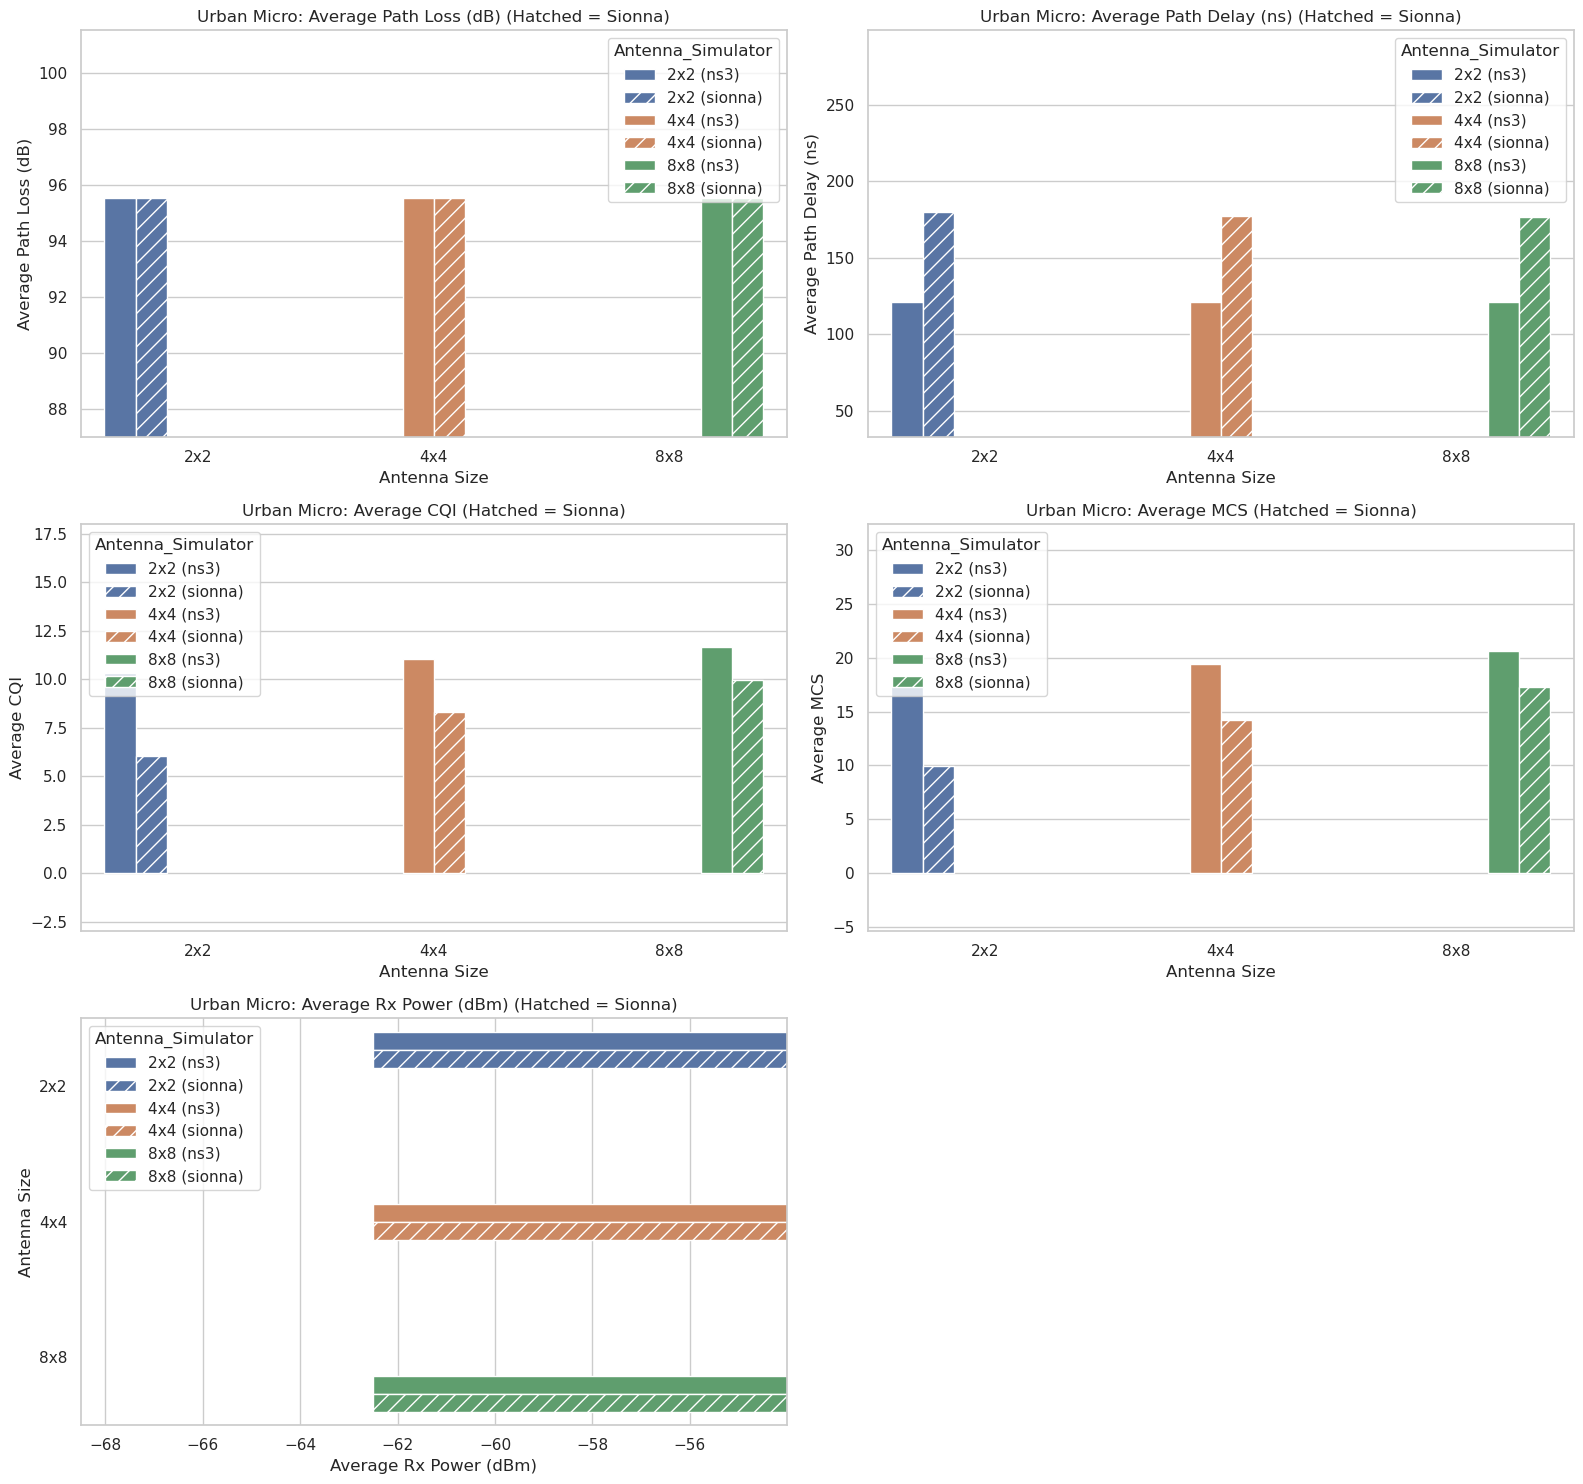
\includegraphics[width=\textwidth]{images/urban_micro_propagation_metrics.png}
    \caption{Urban micro propagation-related metrics by channel mode and gNB array size.}
    \label{fig:exp2-urban-micro-propagation}
\end{figure*}


\subsubsection{Energy Consumption-related Metrics}
\label{subsubsec:exp2-urban-micro-energy}

In Figure \ref{fig:exp2-urban-micro-energy}, the energy consumptions of gNB and UEs by array size, and traffic load are presented.
The gNB energy scaling pattern mirrors the macro scenario: power increases with both array size and traffic load, and Sionna~RT reports slightly lower consumption than ns-3 under high load due to its lower CQI/MCS estimates altering resource allocation.
Under low load, both simulators report $23$~W, $33$~W, and $68$~W for $2\times2$, $4\times4$, and $8\times8$ respectively.
The urban micro scenario adds a notable high-load extreme: the $8\times8$ configuration reaches $215$~W (ns-3) and $193$~W (Sionna~RT) — roughly three times the macro high-load figure — driven by the combined demand of a 400~MHz mmWave channel and dense multipath-induced retransmissions.

UE power consumption ($0.05$~W at low load, $0.09$~W at high load) is nearly identical between the two simulators and independent of gNB array size, confirming that UEs are operating at near-maximum transmit power against the challenging urban channel regardless of the gNB configuration.

\begin{figure*}[t]
    \centering
    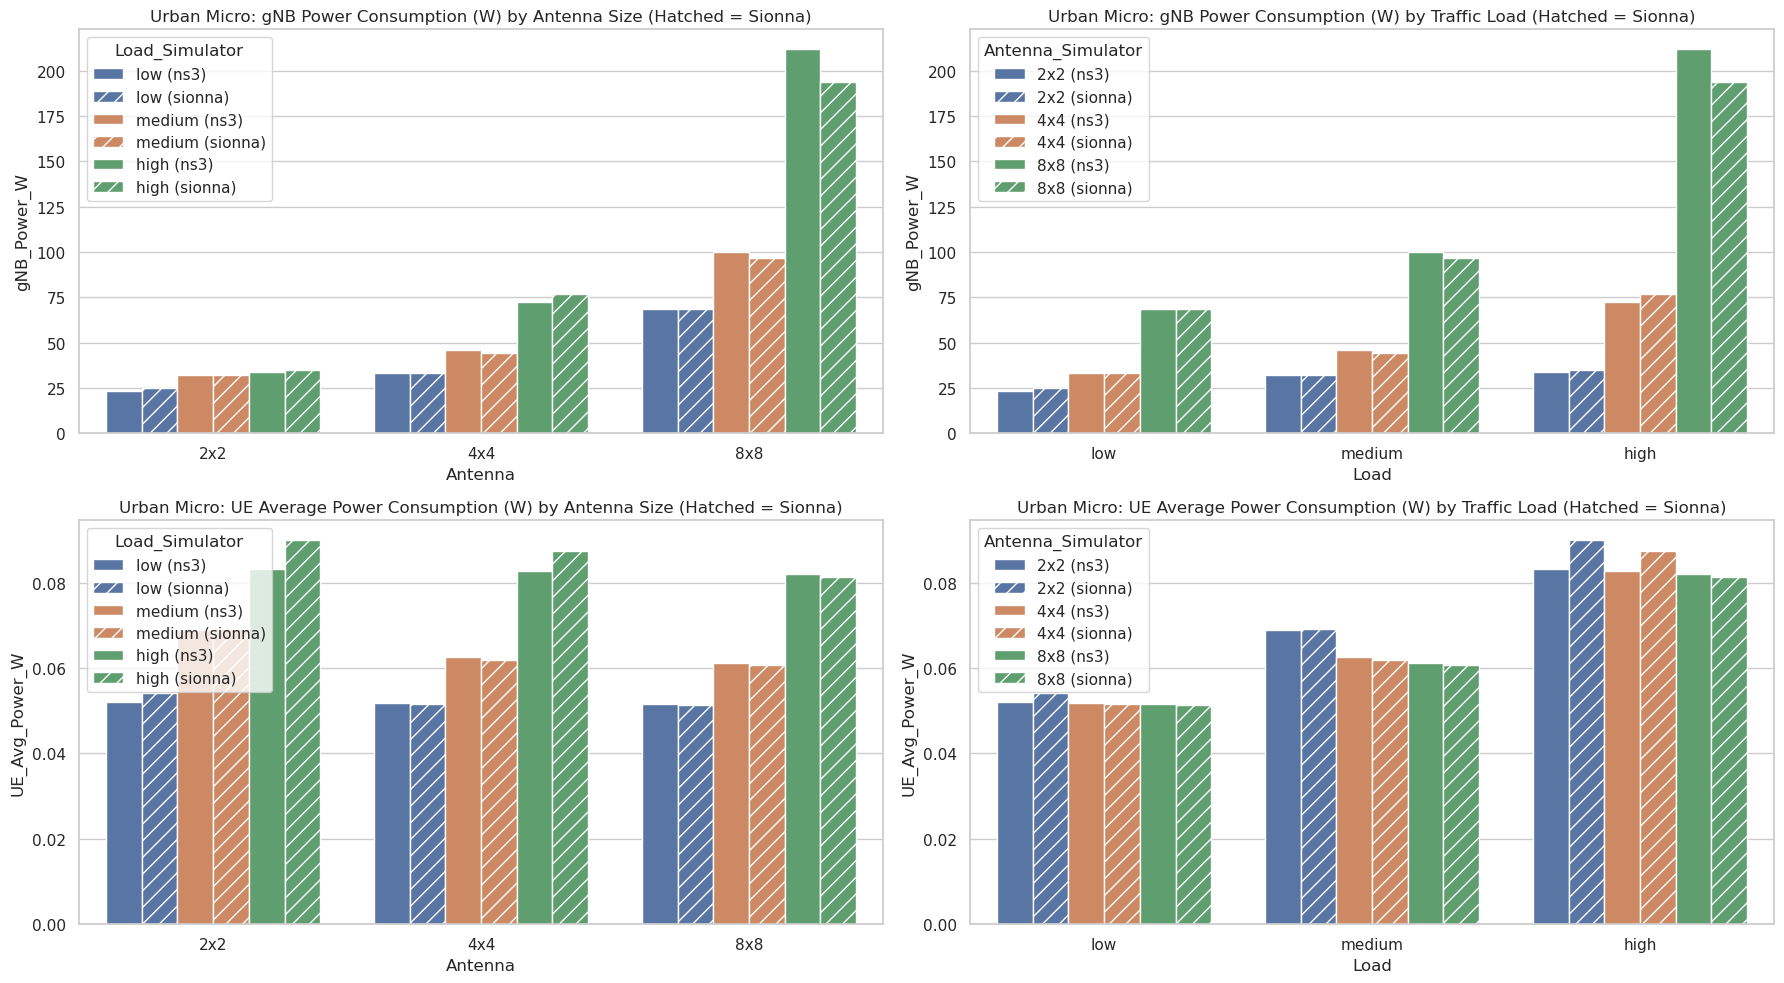
\includegraphics[width=\textwidth]{images/urban_micro_power_consumption.png}
    \caption{Urban micro energy consumptions of gNB and UEs by array size, and traffic load.}
    \label{fig:exp2-urban-micro-energy}
\end{figure*}


\begin{figure*}[t]
    \centering
    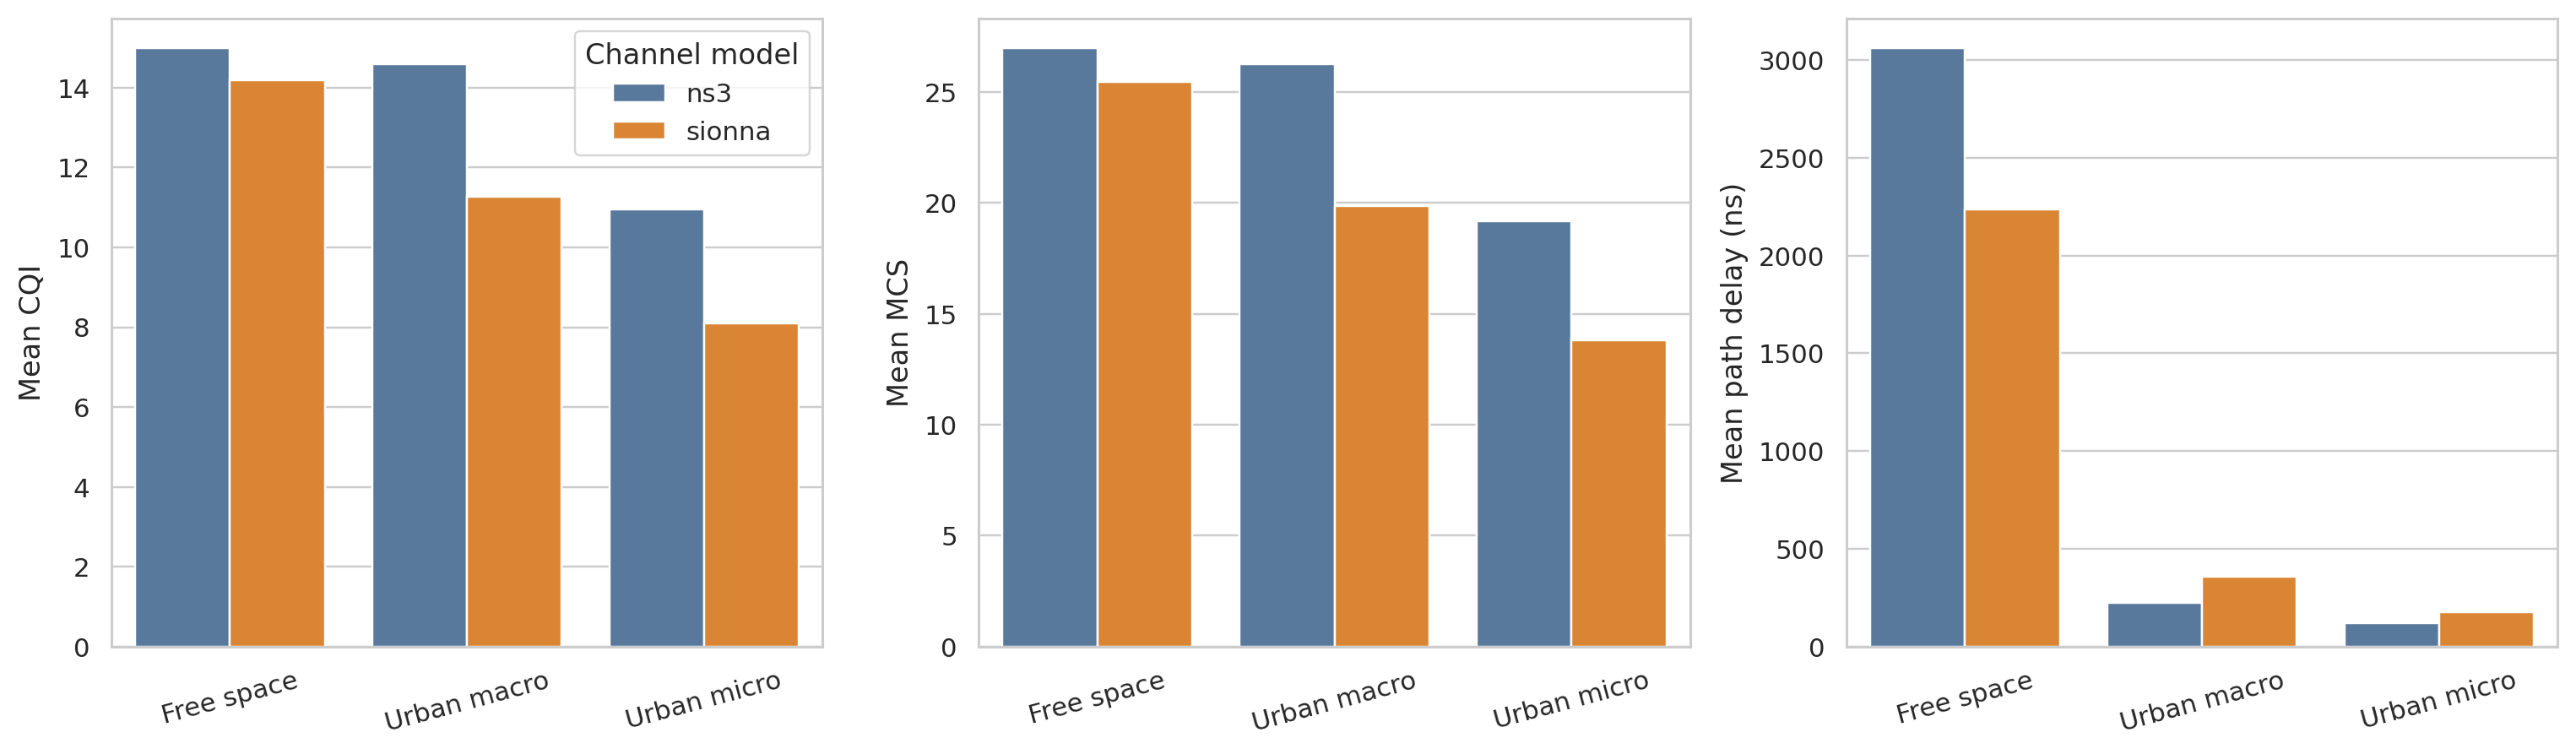
\includegraphics[width=\textwidth]{images/channel_quality_comparison.png}
    \caption{Propagation-related metrics (path loss, received power, path delay, CQI, MCS) across three radio environments and gNB array sizes, comparing ns-3 and Sionna~RT under high traffic load.}
    \label{fig:exp2-channel-quality}
\end{figure*}

\begin{figure*}[t]
    \centering
    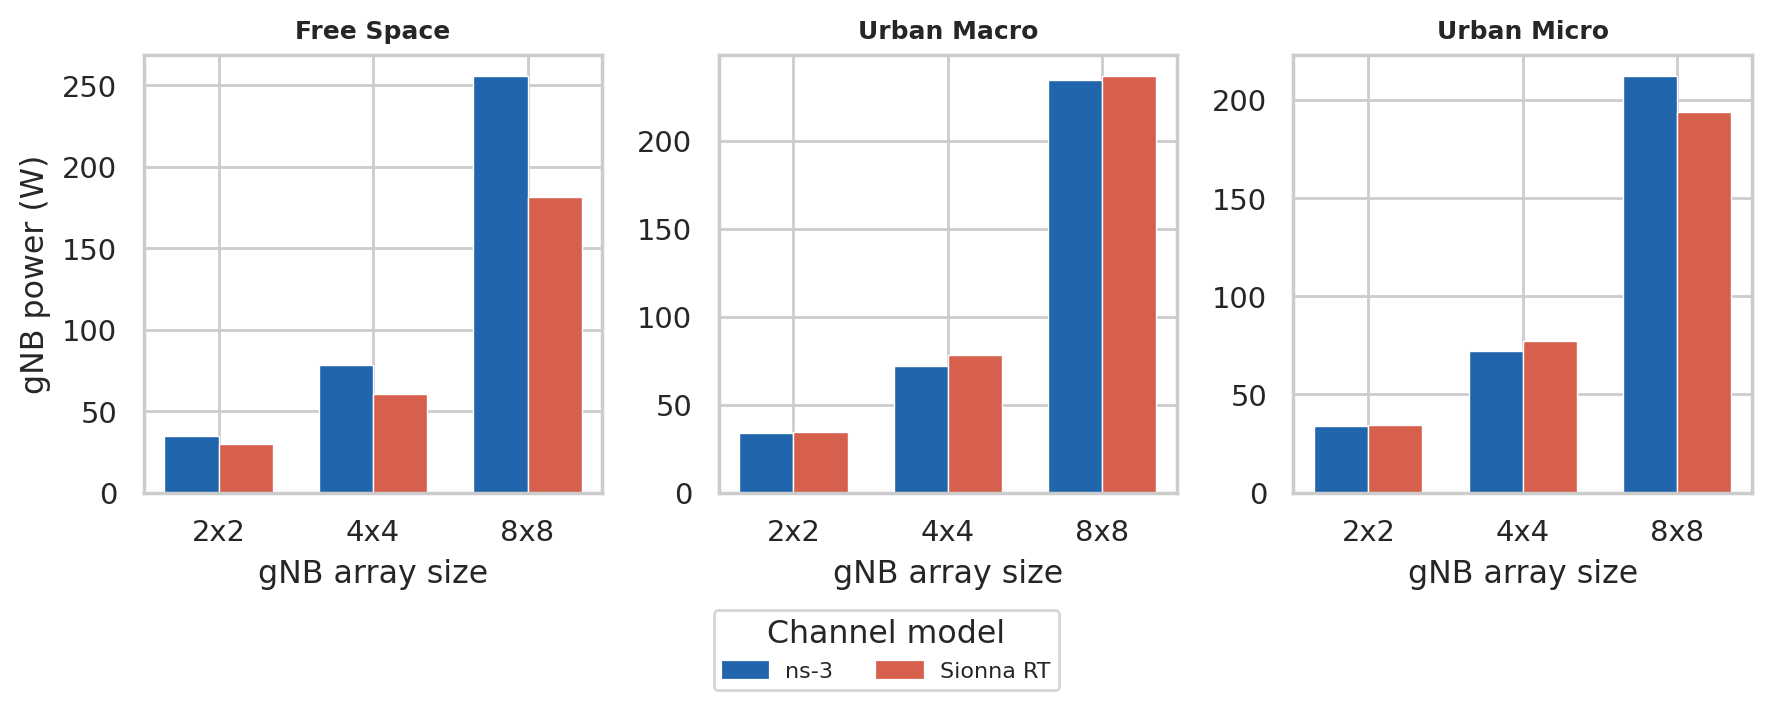
\includegraphics[width=\textwidth]{images/gnb_power_comparison.png}
    \caption{gNB power consumption (W) by array size and radio environment, comparing ns-3 and Sionna~RT under high traffic load.}
    \label{fig:exp2-gnb-power}
\end{figure*}


\section{Conclusion}
\label{sec:conclusion}

This paper presented \texttt{sionnart}: a pybind11-embedded integration of the Sionna~RT ray tracing engine into ns-3, augmented by a displacement-based coherence cache and a proactive adaptive virtual receiver mechanism, both designed to keep per-step GPU overhead manageable.
The embedded design achieves up to $232\times$ lower runtime than the two-process \texttt{ns3sionna} baseline, maintains a GPU memory footprint below 500~MiB, and in stationary scenarios outperforms even the analytical Friis baseline owing to cache-driven elimination of repeated ray tracing calls.
Applied to a 3GPP~NR deployment across free-space, urban macro, and urban micro environments, the framework shows that a geometry-aware channel model produces more conservative — and physically more detailed — channel quality estimates than stochastic models, and confirms that $8\times8$ gNB antenna arrays are essential for overcoming harsh propagation conditions.
As future work, the site-specific multipath data produced by \texttt{sionnart} will be used to extend the framework toward Integrated Sensing and Communications (ISAC) evaluation, enabling joint simulation of communication and sensing within a single ns-3 experiment.

% \begin{thebibliography}{10}

%     \bibitem{sionna}
%     J. Hoydis \emph{et al.}, ``Sionna: An Open-Source Library for Next-Generation Physical Layer Research,'' NVIDIA Research, \url{https://nvlabs.github.io/sionna/}.

%     \bibitem{lena}
%     N. Patriciello \emph{et al.}, ``An E2E Simulator for 5G NR Networks,'' \emph{Simulation Modelling Practice and Theory}, 2019. (5G LENA, CTTC.)

%     \bibitem{tr38901}
%     3GPP TR 38.901, ``Study on Channel Model for Frequencies from 0.5 to 100 GHz,'' v17.0.0, 2022.

%     \bibitem{omnet}
%     A. Varga and R. Hornig, ``An Overview of the OMNeT++ Simulation Environment,'' in \emph{SIMUTools}, 2008.


%     \bibitem{ns3sionna}
%     ``ns3sionna: ns-3 Coupling with Sionna RT via ZMQ,'' open-source project (placeholder reference).

%     \bibitem{pybind11}
%     W. Jakob \emph{et al.}, ``pybind11 -- Seamless Operability between C++11 and Python,'' \url{https://github.com/pybind/pybind11}.

%     \bibitem{eesm}
%     P. Mogensen \emph{et al.}, ``LTE Capacity Compared to the Shannon Bound,'' in \emph{IEEE VTC}, 2007. (EESM link-to-system mapping.)

%     \bibitem{simu5g}
%     G. Nardini, D. Sabella, G. Stea, P. Thakkar, and A. Virdis,
%     "Simu5G--An OMNeT++ Library for End-to-End Performance Evaluation of 5G Networks",
%     \emph{IEEE Access}, vol. 8, pp. 204217-204230, 2020.
%     \url{https://doi.org/10.1109/ACCESS.2020.3035939}

%     \bibitem{ns3}
%     The ns-3 Consortium, ``ns-3 Network Simulator,'' \url{https://www.nsnam.org/}.

%     \bibitem{5glena}
%     N. Patriciello, S. Lagen, B. Bojovic, and L. Gipponi,
%     "An E2E Simulator for 5G NR Networks",
%     \emph{Simulation Modelling Practice and Theory}, vol. 91, pp. 221-231, 2019.
%     \url{https://doi.org/10.1016/j.simpat.2019.101933}

%     \bibitem{sionnart}
%     J. Hoydis, M. Nimier-David, B. Nicolet, S. Cammerer, and A. Keller,
%     "Sionna RT: Technical Report,"
%     \textit{arXiv preprint arXiv:2504.21719},
%     Nov. 2025. [Online]. Available: https://arxiv.org/abs/2504.21719

%     \bibitem{zubow2024ns3-preprint}
%     A. Zubow, Y. Pilz, S. R{\"{o}}sler, and F. Dressler, ``Ns3 meets Sionna: Using Realistic Channels in Network Simulation,'' \textit{arXiv preprint arXiv:2412.20524}, Dec. 2024. [Online]. Available: \url{https://doi.org/10.48550/arXiv.2412.20524}

%     \bibitem{ericson}
%     Ericsson, ``Ericsson Mobility Report,'' Nov. 2025. [Online]. Available: \url{https://www.ericsson.com/4aca6f/assets/local/reports-papers/mobility-report/documents/2025/ericsson-mobility-report-november-2025.pdf}

% \end{thebibliography}

\begin{thebibliography}{99}

    \bibitem{sionna}
    J. Hoydis \emph{et al.}, ``Sionna: An Open-Source Library for Next-Generation Physical Layer Research,'' NVIDIA Research. [Online]. Available: \url{https://nvlabs.github.io/sionna/}

    \bibitem{sionnart}
    F. Ait Aoudia, J. Hoydis, M. Nimier-David \emph{et al.},
    ``Sionna RT: Technical Report,''
    \emph{arXiv preprint arXiv:2504.21719}, 2025.
    doi: \url{https://doi.org/10.48550/arXiv.2504.21719}

    \bibitem{ns3}
    The ns-3 Consortium, ``ns-3 Network Simulator.'' [Online]. Available:
    \url{https://www.nsnam.org/}

    \bibitem{5glena}
    N. Patriciello, S. Lagen, B. Bojovic, and L. Giupponi,
    ``An E2E Simulator for 5G NR Networks,''
    \emph{Simulation Modelling Practice and Theory}, vol. 96, p. 101933, 2019.
    doi: \url{https://doi.org/10.1016/j.simpat.2019.101933}

    \bibitem{tr38901}
    3GPP, ``Study on Channel Model for Frequencies from 0.5 to 100 GHz,''
    3GPP TR 38.901, v17.0.0, 2022.

    \bibitem{omnet}
    A. Varga and R. Hornig,
    ``An Overview of the OMNeT++ Simulation Environment,''
    in \emph{Proceedings of the 1st International Conference on Simulation Tools and Techniques for Communications, Networks and Systems (SIMUTools)}, 2008.

    \bibitem{simu5g}
    G. Nardini, D. Sabella, G. Stea, P. Thakkar, and A. Virdis,
    ``Simu5G--An OMNeT++ Library for End-to-End Performance Evaluation of 5G Networks,''
    \emph{IEEE Access}, vol. 8, pp. 181176--181191, 2020.
    doi: \url{https://doi.org/10.1109/ACCESS.2020.3028550}

    \bibitem{ns3sionna}
    A. Zubow, Y. Pilz, S. R{\"o}sler, and F. Dressler,
    ``Ns3 Meets Sionna: Using Realistic Channels in Network Simulation,''
    \emph{arXiv preprint arXiv:2412.20524}, 2024.
    doi: \url{https://doi.org/10.48550/arXiv.2412.20524}

    \bibitem{pybind11}
    W. Jakob, J. Rhinelander, and D. Moldovan,
    ``pybind11 -- Seamless Operability between C++11 and Python.'' [Online].
    Available: \url{https://github.com/pybind/pybind11}

    \bibitem{eesm}
    P. Mogensen \emph{et al.},
    ``LTE Capacity Compared to the Shannon Bound,''
    in \emph{Proceedings of the IEEE Vehicular Technology Conference (VTC)}, 2007.

    \bibitem{bojovic_mimo}
    B. Bojovic, Z. Ali, S. Lagen, and L. Giupponi,
    ``ns-3 and 5G-LENA Extensions to Support Dual-Polarized MIMO,''
    in \emph{Proceedings of the Workshop on ns-3}, 2022, pp. 1--9.
    doi: \url{https://doi.org/10.1145/3532577.3532595}

    \bibitem{bojovic_beamforming}
    B. Bojovic, S. Lagen, and L. Giupponi,
    ``Realistic Beamforming Design Using SRS-Based Channel Estimate for ns-3 5G-LENA Module,''
    in \emph{Proceedings of the Workshop on ns-3}, 2021, pp. 81--87.
    doi: \url{https://doi.org/10.1145/3460797.3460809}

    \bibitem{raymobtime_sionna}
    S. Bastos, A. P. Oliveira, and D. T. Suzuki,
    ``Generation of 5G/6G Wireless Channels Using Raymobtime with Sionna's Ray-Tracing,''
    in \emph{Proceedings of the Brazilian Telecommunications and Signal Processing Symposium}, 2023.
    doi: \url{https://doi.org/10.14209/sbrt.2023.1570923823}

    \bibitem{alsamman_mmwave}
    A. M. Al-Samman, M. Cheffena, O. Elijah, Y. A. Al-Gumaei, S. K. Abdul Rahim, and T. A. Rahman,
    ``Survey of Millimeter-Wave Propagation Measurements and Models in Indoor Environments,''
    \emph{Electronics}, vol. 10, no. 14, p. 1653, 2021.
    doi: \url{https://doi.org/10.3390/electronics10141653}

    \bibitem{han_thz}
    C. Han, Y. Wang, and Y. Li,
    ``Terahertz Wireless Channels: A Holistic Survey on Measurement, Modeling, and Analysis,''
    \emph{arXiv preprint arXiv:2111.04522}, 2021.
    doi: \url{https://doi.org/10.48550/arXiv.2111.04522}

    \bibitem{uwaechia_mmwave}
    A. N. Uwaechia and N. M. Mahyuddin,
    ``A Comprehensive Survey on Millimeter Wave Communications for Fifth-Generation Wireless Networks: Feasibility and Challenges,''
    \emph{IEEE Access}, vol. 8, pp. 62367--62414, 2020.
    doi: \url{https://doi.org/10.1109/ACCESS.2020.2984204}

    \bibitem{cazzella_dt_mimo}
    L. Cazzella, D. Tagliaferri, and M. Mizmizi,
    ``Deep Learning of Transferable MIMO Channel Modes for 6G V2X Communications,''
    \emph{IEEE Transactions on Antennas and Propagation}, vol. 70, no. 6, pp. 4127--4139, 2022.
    doi: \url{https://doi.org/10.1109/TAP.2022.3169950}

    \bibitem{zhou_isac}
    W. Zhou, R. Zhang, G. Chen, and W. Wu,
    ``Integrated Sensing and Communication Waveform Design: A Survey,''
    \emph{IEEE Open Journal of the Communications Society}, vol. 3, pp. 1930--1949, 2022.
    doi: \url{https://doi.org/10.1109/OJCOMS.2022.3215683}

    \bibitem{gao_isac_mimo}
    Z. Gao, Z. Wan, D. Zheng, M. Matthaiou, and B. Ai,
    ``Integrated Sensing and Communication With mmWave Massive MIMO: A Compressed Sampling Perspective,''
    \emph{IEEE Transactions on Wireless Communications}, vol. 22, no. 3, pp. 1745--1762, 2023.
    doi: \url{https://doi.org/10.1109/TWC.2022.3206614}

    \bibitem{hua_isac_beamforming}
    H. Hua, J. Xu, and T. X. Han,
    ``Optimal Transmit Beamforming for Integrated Sensing and Communication,''
    \emph{arXiv preprint arXiv:2104.11871}, 2021.
    doi: \url{https://doi.org/10.48550/arXiv.2104.11871}

    \bibitem{samorzewski_energy}
    A. Samorzewski, M. Deruyck, and A. Kliks,
    ``Energy Consumption in RES-Aware 5G Networks,''
    in \emph{Proceedings of IEEE Global Communications Conference (GLOBECOM)}, 2023, pp. 1024--1029.
    doi: \url{https://doi.org/10.1109/GLOBECOM54140.2023.10437451}

    \bibitem{ericsson_mobility}
    Ericsson, ``Ericsson Mobility Report,'' Nov. 2025. [Online]. Available:
    \url{https://www.ericsson.com/4aca6f/assets/local/reports-papers/mobility-report/documents/2025/ericsson-mobility-report-november-2025.pdf}

\end{thebibliography}


% \input{07_Biography/biography.tex}

\end{document}